% Draft stages:
% outline - Basic layout and section design
% draft alpha - Information for all sections in a vaguely structured format
% draft beta - All sections revised into actual sentences
% draft 0 - Chapter has all information with proper sentence structure and section transitions, along with needed figures
% draft # - Anything after revising the #th series of comments from Steve
% draft omega # - Anything after revising the #th series of comments from the committee/higher bureaucracy
\documentclass[12pt]{report}

\usepackage{Dedman-Thesis-Latex-Template/sty/DL_thesis}  % Global Style for particular SMU College, e.g. DL_thesis.sty
\input{Dedman-Thesis-Latex-Template/latex/packages.tex}
% Load additional packages here.
% Be careful of the loading order with respect to packages.tex as conflicts can easily arise.
% This is not a part of the base template and so will never be overwritten during updates.
\usepackage{tikz}
\usepackage{graphicx}
\usepackage{tikz-feynman}
\usepackage{fontspec}
%\usepackage{mathtools}
\newfontface\mathcursivefont{Daytonia.otf}
\DeclareTextFontCommand{\mathcurse}{\mathcursivefont}
 % Uncomment to load additional user required packages
\input{Dedman-Thesis-Latex-Template/latex/preamble.tex}
\input{Dedman-Thesis-Latex-Template/latex/custom_commands.tex}
% Place your own personal commands here. 
% This is not a part of the base template and so will never be overwritten during updates.
 % Uncomment to use your own personal commands
\AuthorFirstName{Graduate}
\AuthorLastName{Student}
% \AuthorNameSuffix{Jr.}

% Title can be up to three lines of no more than 48 characters per line
% Write the title with the capitalization you want to be used in the abstract
\ThesisTitle{Smashy Physics:}{How I Pretended to Do More Smashing}{Using Smashy Math}
\GraduateDepartment{Physics}

\FirstDegree%
\FirstDegreeType{B.S.}
\FirstDegreeMajor{Physics}
\FirstDegreeUniversity{Undergraduate University}

\SecondDegree%
\SecondDegreeType{M.S.}
\SecondDegreeMajor{Physics}
\SecondDegreeUniversity{Southern Methodist University}

\ThesisDefenseDateYear{2022}
\ThesisDefenseDateMonth{April}
\ThesisDefenseDateDay{1}

\GraduationDateYear{2022}
\GraduationDateMonth{July}
\GraduationDateDay{1}

\SMUCollege{Dedman College}

% Committee
\AdvisorFullName{Dr.~Stephen Sekula}
\AdvisorTitle{Associate Professor}

\CommitteeMemberA{Dr.~Roberto Vega}
\CommitteeMemberTitleA{Professor}

\CommitteeMemberB{Dr.~Jingbo Ye}
\CommitteeMemberTitleB{Associate Professor}

\CommitteeMemberC{Dr.~External Member}
\CommitteeMemberTitleC{Assistant Professor}

\hypersetup{
 % Added more precise definition and options for Hyperref package.
 % Comment out or change hyperref preferences
 % \hypersetup should be loaded last
 bookmarksopen=true, % True: Open bookmark tree
 bookmarksnumbered=true, % True: put section numbers in bookmarks
 breaklinks=true, % True: split the url over multiple lines
 %   draft=true, % True: do not do any hyper linking
 filecolor=magenta, % Color of file links
 citecolor=blue, % Color of links to bibliography
 colorlinks=true, % False: boxed links; true: colored links
 linkcolor=blue, % Color of internal links
 linktocpage=true, % True: Makes the page number of TOC the link vs the text
 %   pagebackref=true, % True: Links references back to referring page
 pdfnewwindow=true, % True: URL links in new window
 plainpages=false, % True: do page number anchors as plain Arabic
 pdffitwindow=false, % Window fit to page when opened
 pdfmenubar=true, % Show Acrobat menu
 pdfstartview={FitH}, % Fits the width of the page to the window
 pdftoolbar=true, % Show Acrobat toolbar
 pdfauthor={Author}, % Author in PDF document properties
 pdfcreator={Author}, % Creator of the document in PDF document properties
 pdfkeywords={Keyword1} {Keyword2} {Keyword3} {Keyword4} {Author}, % List of keywords in PDF document properties
 pdfproducer={Producer}, % Producer of the document in PDF document properties
 pdfsubject={Subject}, % Subject of the document in PDF document properties
 pdftitle={Title of Dissertation}, % Title in PDF document properties
 unicode=false, % Non-Latin characters in Acrobat bookmarks
 urlcolor=cyan % Color of external links
}


\makeglossaries
\newglossaryentry{LHC}{
 text=LHC,
 long=Large Hadron Collider,
 name={\glsentrylong{LHC} (\glsentrytext{LHC})},
 first={\glsentryname{LHC}},
 sort={large hadron collider},
 description={Large Hadron Collider}
}

\newglossaryentry{thesis}{
 name=thesis,
 description={https://xkcd.com/1403/}
}


% \thesisdraft % uncomment if want draft printing

\begin{document}

\input{Dedman-Thesis-Latex-Template/latex/front_pages.tex} %TODO

\begin{thesis}

%\chapter*{Preface}\label{chapter:preface}
% c.f. https://tex.stackexchange.com/a/222961/152544
\addcontentsline{toc}{chapter}{\protect\numberline{}Preface}

The following is a summary of useful concepts in high energy particle physics.

\section{Units}\label{section:units}

Discussion of units

\section{Coordinates}\label{section:coordinates}

\gls{LHC} coordinate systems

\section{Statistics}\label{section:statistics}

Statistics in particle physics
 %TODO

% Ch1: I'll deal with this later
%\chapter{Introduction}\label{chapter:introduction}

%The basic structure of every lab report you've ever done is: 
%    introduction,
%    theory,
%    experimental setup,
%    procedure,
%    results,
%    conclusion.
%
%This thesis is essentially following that same format:
%    Introduction,
%    Standard Model... and Signal modelling? (theory),
%    LHC and ATLAS and Trigger (experimental setup)
%    Reconstruction, Selection, Background Estimation (procedure)
%    results (...)
%    conclusion

The Higgs Boson was proposed as a fundamental particle in 1964,
    and has been a driving factor in particle physics research ever since.
Though it was jointly discovered in 2012 by the ATLAS and CMS collaborations,
    there are still a number of properties of the Higgs which have yet to be measured.
Chief among these are two of the Higgs' self-coupling constants, \kl and \kvv,
    which determine how strongly the Higgs interacts with both itself and with vector bosons.
This analysis performs a search for the rare,
    as-yet unseen diHiggs interaction in order to set tighter constraints on these coupling values.
The search utilizes the Vector Boson Fusion production mechanism of the diHiggs process,
    identifying the process in the 4b final state.
This is performed using 126 $\textit{fb}^{-1}$ of data from Run 2 of ATLAS.

This thesis will begin by first explaining the importance of the Higgs Boson to the field of particle physics,
    as well as the relevance of the aforementioned \kl and \kvv coupling constants.
I will then describe the physical effects of these constants,
    and how those effects can be exploited in order to make measurements of them.
These topics comprise Chapter \ref{chapter:theory}.
Following from the theoretical discussion, I will discus the experimental equipment and setup used to perform the  measurments.
The experimental setup is discussed across three chapters.
Chapter \ref{chapter:lhc} discusses the Large Hadron Collider, the machine which generates the conditions necessary to produce diHiggs process.
Actual observation of the process once generated is carried out by the ATLAS particle detector array and its Trigger system,
    described in Chapters \ref{chapter:atlas} and \ref{chapter:trigger}.
The reconstruction process, described in Chapter \ref{chapter:reconstruction},
    entails how data observed by ATLAS is analyzed in order to determine which physics processes occured during the myriad observed interactions.
Background processes are removed from the data set using a selection procedure explained in Chapter \ref{chapter:selection},
    and the contribution of the background events which remain is estimated using data-driven technique cataloged in Chapter \ref{chapter:background}. 
The background estimation process makes use of a neural network reweighting procedure, which I personally configured and ran the training for.
My primary contribution to the analysis however, comes in the form of the signal model that constitutes the hypothesis for the behaviour of the Higgs Boson.
The signal model makes use of a Monte-Carlo sample combination technique, which I developed and optimized in the context of the \vbfproc process.
This is elaborated upon in Chapter \ref{chapter:signal}.
Finally, in Chapter \ref{chapter:results}, this hypothesis alongside the background estimate are compared against the data observed from ATLAS,
    in order to make constraints on the diHiggs self-coupling constants.



%This is the first chapter of the \gls{thesis}.~\cite{Aaboud:2016mmw,Bruning:782076}

\section{Creating Figures}\label{sec:figures}
\begin{figure}[htpb]
 \centering
 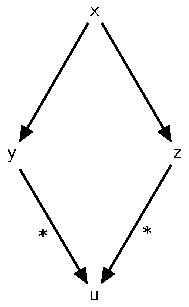
\includegraphics{introduction/example.pdf}
 \caption[Example placeholder figure with a citation~\cite{Higgs:1964ia} and shorter List of Figures caption.
  The List of Figures is protected from first use of glossary entries or acronyms like \acrlong{LHC}.]{%
  This is a placeholder figure to act as an example.
  Here we cite a new reference in the caption to demonstrate that given the package configuration our order of references will not be distributed by the table of contents~\cite{Higgs:1964ia}.}\label{fig:test_figure}
\end{figure}

As can be seen in \Cref{fig:subfigure_example}, the subfigures are independent of each other such that \Cref{fig:subfigure_1} and \Cref{fig:subfigure_2} can be accessed separately.

\begin{figure}[htbp]
 \centering
 \begin{subfigure}[t]{0.48\textwidth}
  \centering
  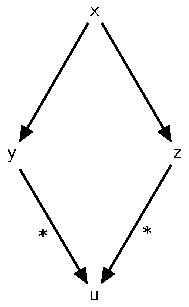
\includegraphics[width=0.3\textwidth]{introduction/example.pdf}
  \caption[Short List of Figures captions work with subfigures too.]{%
   This is the first figure of two, in this example, and its own independent subfigure.}
  \label{fig:subfigure_1}
 \end{subfigure}%
 \quad
 \begin{subfigure}[t]{0.48\textwidth}
  \centering
  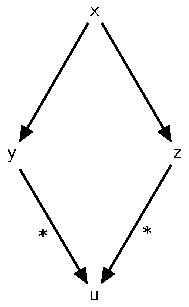
\includegraphics[width=0.3\textwidth]{introduction/example.pdf}
  \caption[Which makes the List of Figures readable and actually helpful.]{%
   As the \texttt{t} alignment option was chosen for the subfigures, they are still properly aligned vertically even though this caption is longer.}
  \label{fig:subfigure_2}
 \end{subfigure}
 \caption{An example of a figure that consists of two subfigures.}
 \label{fig:subfigure_example}
\end{figure}

As an example of an equation formatted in ``\href{https://www.overleaf.com/learn/latex/Display_style_in_math_mode}{display style}'' the equation for the fiducial cross section from~\cite{Aaboud:2016mmw} is reproduced as \Cref{eq:fiducial_cross_section}:
\begin{equation}
 \sigma_{\mathrm{inel}}^{\mathrm{fid}} \left(\zeta > 10^{-6}\right) = \frac{N - N_{\mathrm{BG}}}{\epsilon_{\mathrm{trig}} \times \mathcal{L}} \times \frac{1 - f_{\zeta < 10^{-6}}}{\epsilon_{\mathrm{sel}}}
 \label{eq:fiducial_cross_section}
\end{equation}

\section{Creating Tables}\label{sec:tables}

To create tables in \LaTeX{} it is highly recommended to use the \href{https://www.ctan.org/pkg/booktabs}{\texttt{booktabs}} package.
It allows for very elegant and clean table creation, such as \Cref{table:natural_units}.
If you want to create a table quickly, or have a CSV file that you'd like to quickly turn into a table there are various \href{https://www.tablesgenerator.com/}{online \LaTeX{} table generators}.

\begin{table}[htpb]
 \centering
 \caption[Common quantities in particle physics in natural and SI units.]{%
  Common quantities in particle physics given in both natural units and SI units.}
 \begin{tabular}{@{}llll@{}} \toprule
  Quantity         & Natural Units                 & Natural Units (dimensionful)            & SI Units                                              \\ \midrule
  Speed            & $1$                           & $c$                                     & $3.0\times 10^{8}~\mathrm{m}/\mathrm{s}$              \\
  Angular Momentum & $1$                           & $\hbar$                                 & $10^{34}~\mathrm{m}^2 \,\mathrm{kg}/\mathrm{s}$       \\
  Energy           & $\mathrm{GeV}$                & $\mathrm{GeV}$                          & $1.6\times 10^{-10}~\mathrm{J}$                       \\
  Momentum         & $\mathrm{GeV}$                & $\mathrm{GeV}/c$                        & $1\times 10^{-19}~\mathrm{kg}\,\mathrm{m}/\mathrm{s}$ \\
  Mass             & $\mathrm{GeV}$                & $\mathrm{GeV}/c^{2}$                    & $1.8\times 10^{-27}~\mathrm{kg}$                      \\
  Time             & $1/\mathrm{GeV}$              & $\hbar/\mathrm{GeV}$                    & $6.6\time 10^{-25}~\mathrm{s}$                        \\
  Length           & $1/\mathrm{GeV}$              & $\hbar c/\mathrm{GeV}$                  & $2\times 10^{-16}~\mathrm{m}$                         \\
  Electric Charge  & $1$                           & $e/\sqrt{4\pi \alpha_{\mathrm{em}}}$    & $5.3\times 10^{-19}~\mathrm{C}$                       \\
  Magnetic Field   & $\left(\mathrm{GeV}\right)^2$ & $\left(\mathrm{GeV}\right)^2/\hbar c^2$ & $5\times 10^{16}~\mathrm{T}$                          \\
  \bottomrule
 \end{tabular}\label{table:natural_units}%
\end{table}

Good table design requires some thought and work, so it may be worth a look through some examples:
\begin{itemize}
 \item \href{https://tex.stackexchange.com/questions/238503/tip-on-how-to-make-a-visually-good-table}{TeX StackExchange: Tip on how to make a visually good table}
 \item \href{https://twitter.com/edwardtufte/status/451820483109847040?lang=en}{Edward Tufte endorsed} example from \href{http://static1.squarespace.com/static/56713bf4dc5cb41142f28d1f/t/56fd4c83746fb9261146eed5/1459440776291/ClearOffTheTableMd.gif}{Darkhorse Analytics}
\end{itemize}

\section{Dealing with Widows and Orphans}\label{sec:widos_and_orphans}

To reduce the difficulty of dealing with widowed text (the last line of a paragraph at the start of a page) and orphaned text (the first line of paragraph at the end of a page) the \href{https://ctan.org/pkg/nowidow?lang=en}{\texttt{nowidow}} package is used.
However, that doesn't solve the issue of orphaned section titles.
The user must manually do this, but the following \href{https://texfaq.org/FAQ-widows}{simple advice from \TeX{} FAQ} is recommended:

\begin{quote}
 Once you've exhausted the automatic measures, and have a final draft you want to ``polish'', you should proceed to manual measures.
 To get rid of an orphan is simple: precede the paragraph with \texttt{\textbackslash clearpage} and the paragraph can’t start in the wrong place.
\end{quote}

 %TODO: Add to this once you know the structure of the rest

% Ch2: Standard Model Discussion
%\chapter{Theory}\label{chapter:theory}

%So what even do I need to talk about here?
%
%Final goal = Higgs (final goal should actually probably be di-higgs and a discussion of the relevence of this...)
%    What: What is the Higgs?
%    Why: Why do we care about it? It gives things mass and messes with the electroweak interaction
%    When: In what contexts does the Higgs become relevant? The mass of (most) elementary particles and the weak force being weak
%    Where: Where does the higgs fit into the SM? The "Higgs Mechanism"
%    How: How does the higgs mechanism work?

\section{Introduction}

    The Higgs Boson sits as the crown jewel of a grand overarching theory of the behaviour of the universe,
        known as the Standard Model of Particle Physics.
    While its recent discovery has shed light on many of its key properties,
        there are still many details of its nature that are as yet uncomfirmed.
    In this chapter, I want to explain what these properties are and how they can be further studied.
    Moreover, I want to justify why the Higgs is so important as to be worth studying in the first place.
    And to understand the importance of the Higgs Boson, one must understand the structure of the Standard Model itself.

    The structure of the following sections will begin with a discussion of the purpose and fundamental structure of the Standard Model.
    I will follow this with an introduction to the mathematical formalism the Standard Model is based around,
        involving Group Theory, the calculus of variations, and symmetry.
    Here I will introduce the reason for the original postulation of the Higgs, what it is, how it works, and how it fits into the Standard Model.
    Finally, I will motivate further study into the Higgs and provide a technique to perform this study.


%Matter and Forces
%I need to discuss the elementary particles and their organization before I can really discuss the gauge fields.
%Might as well do it here first and foremost
\section{The Standard Model of Particle Physics}
    
    At its core, the Standard Model of Particle Physics is a description of the behaviour and interaction of matter.
    First and foremost then, I want to discuss what this matter actually is.
    All matter can be described as a specific type of elementary particle called a fermion,
        defined by the fact that it contains no discernable substructure and possesses an intrinsic spin of 1/2.
    These particles all have different masses, and are able to interact with each other through three ``fundamental interactions''.
    The three fundamental interactions (more commonly called ``Fundamental Forces'') are known as
        the Electromagnetic, Weak, and Strong interactions (gravity is entirely absent in the Standard Model).
    All the interactions have an associated ``charge'' which can be ascribed to different particles,
        and which govern how strongly that particle can interact with similarly charged particles.
    The various fermions are distinct largely because of the charges they carry.

    \begin{figure}[h!]
        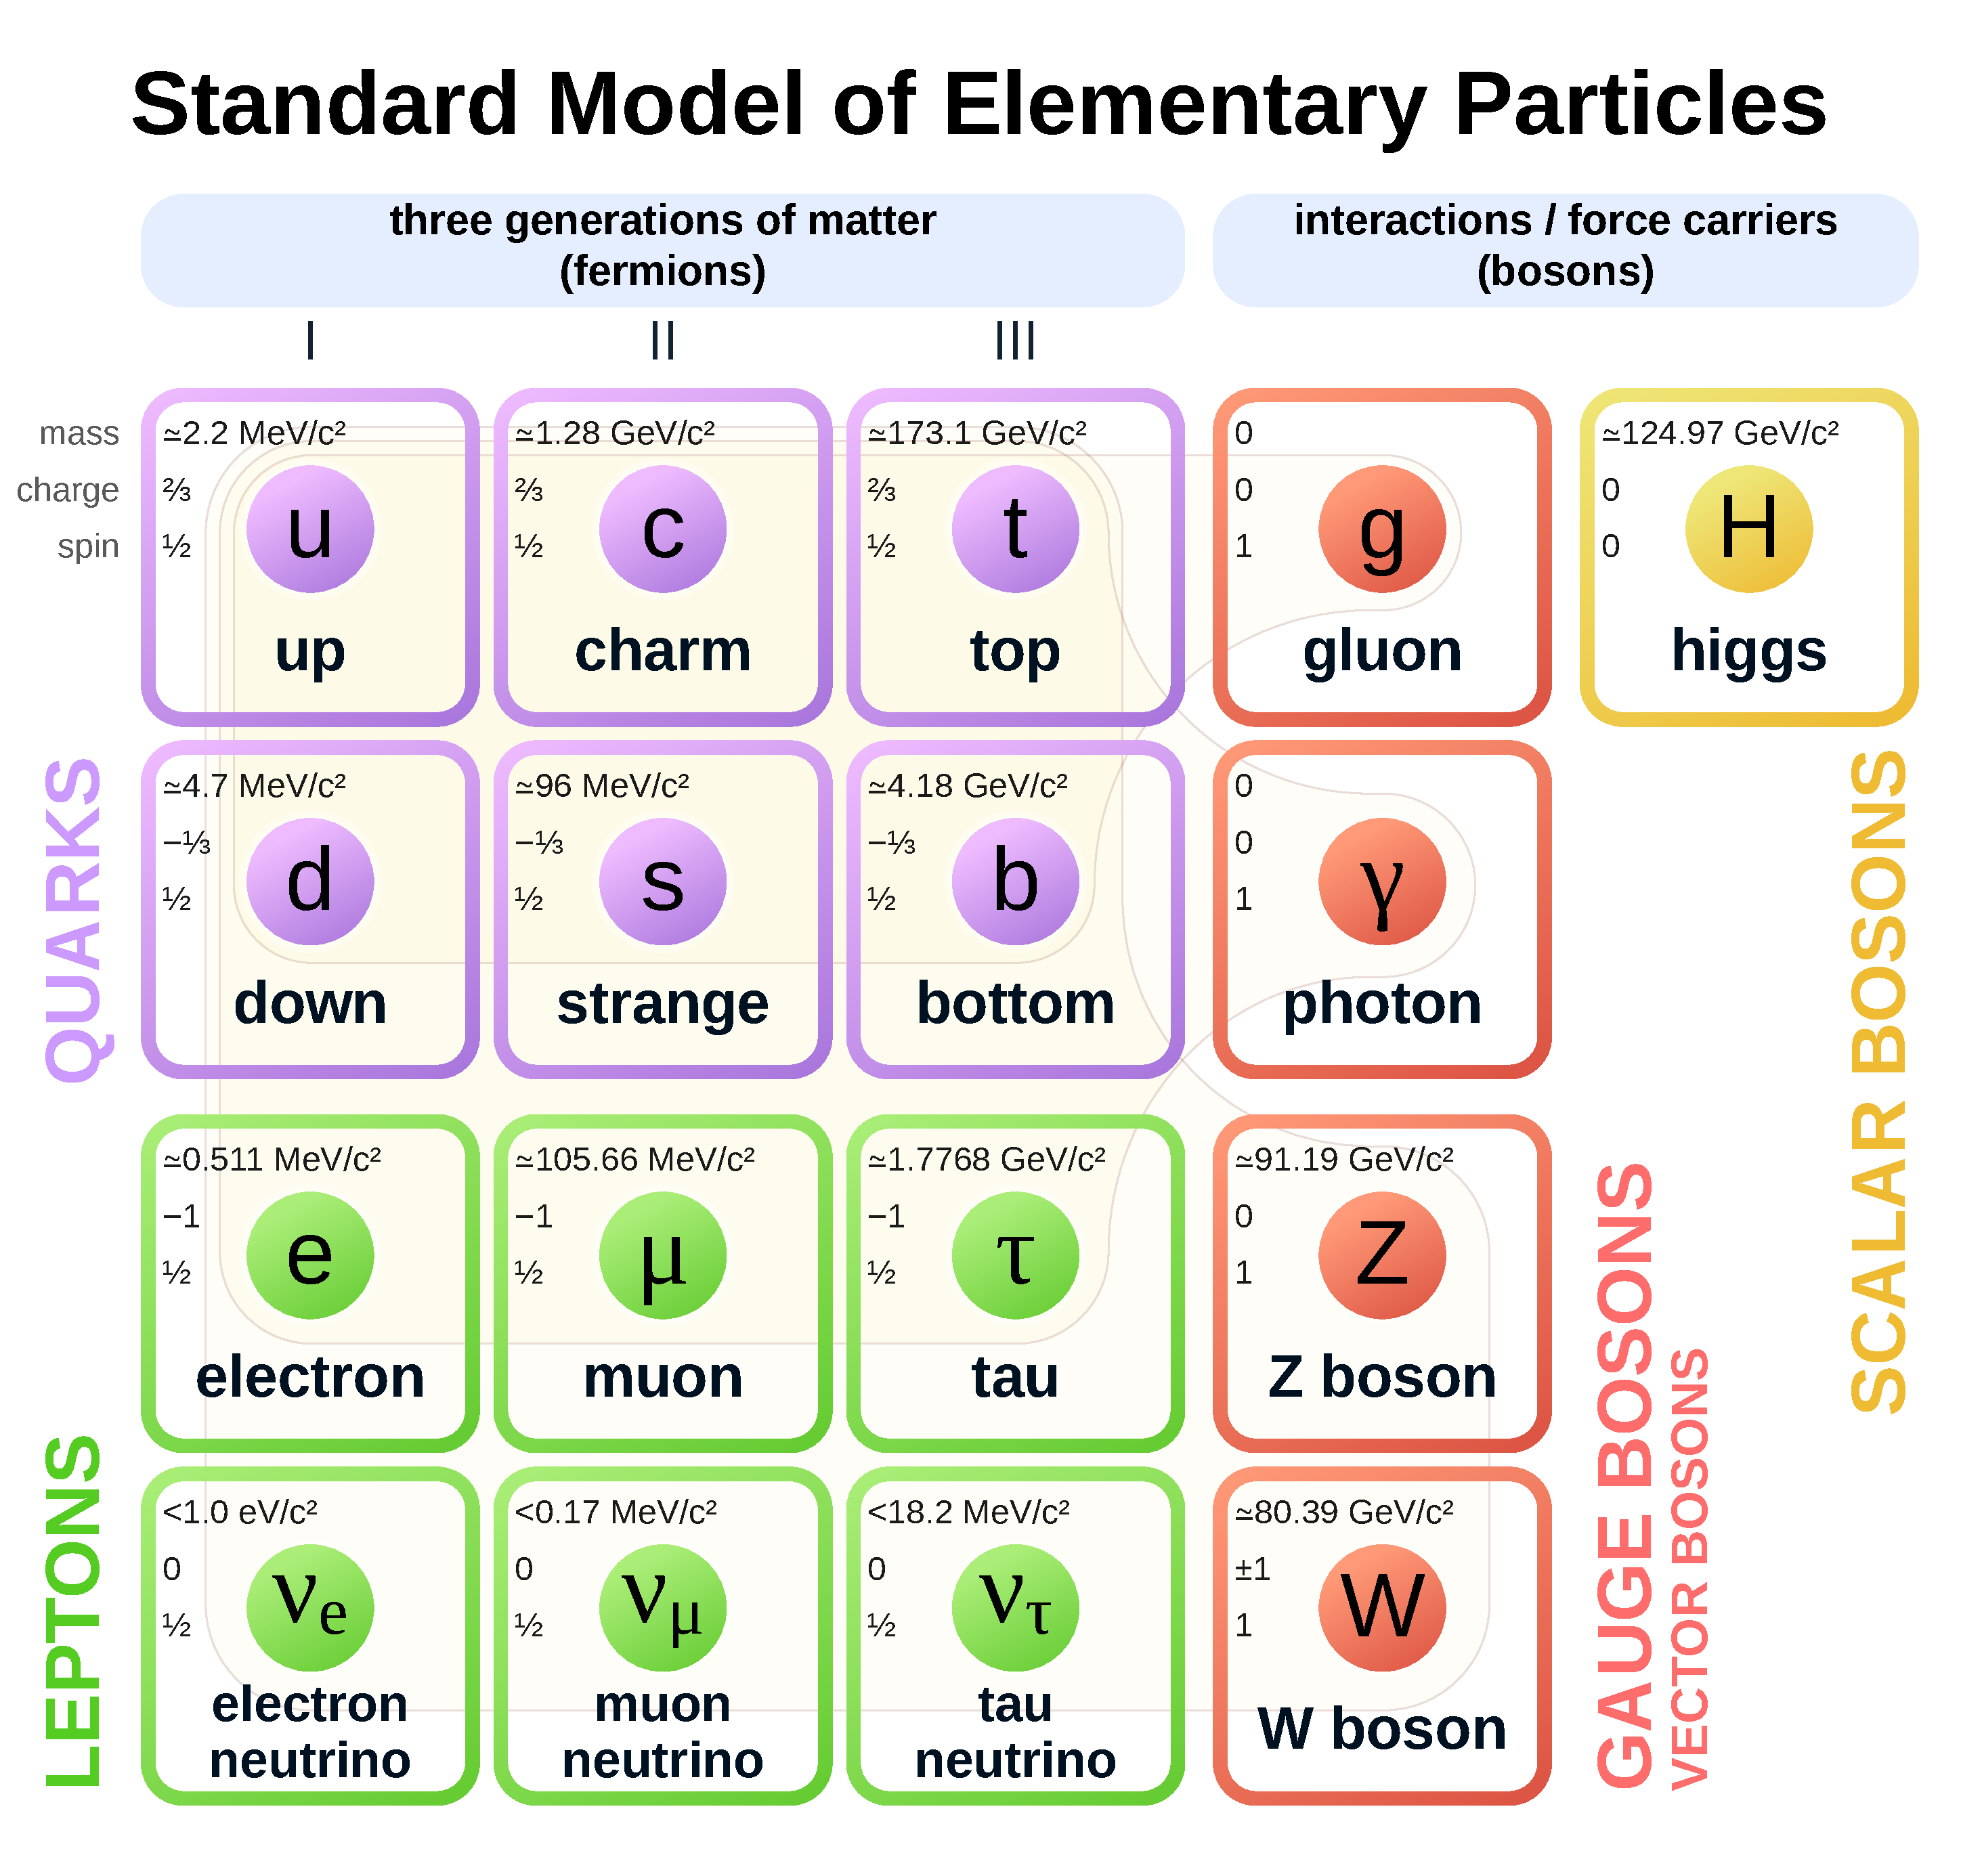
\includegraphics[width=\linewidth,height=\textheight,keepaspectratio]{theory/Standard_Model_of_Elementary_Particles}
        \caption{I'm probably going to need to find something else since this came from wikipedia. I just wanted a placeholder}
        \label{fig:sm_particles}
    \end{figure}
        

    There are twelve distinct elementary fermions (see Figure \ref{fig:sm_particles}),
        which are split evenly into two subgroups, called quarks and leptons.
    Quarks have a charge of 1 with the Strong interaction,
        while leptons have a charge of 0 (and thus cannot interact via the Strong Interaction at all).
    Both classes of particles, quarks and leptons, are divided into three ``generations'' of progressively heavier particles.
    Each generation thus consists of two quarks and two leptons.
    These pairs, called ``doublets'', behave the same across all generations.
    Among the quarks, every generation contains a doublet of an up-type quark (Up, Charm, Top) with electromagnetic charge of 2/3,
        and a down-type quark (Down, Strange, Bottom) with EM charge of -1/3.
    For leptons, each doublet consists of a particle with EM charge of -1, and a neutrino with EM charge of 0.

    In addition to the fermions, there is also an entirely seperate class of particles, called gauge bosons,
        which play a fundamental role in the aforementioned interactions.
    However, the nature of these particles will be discussed later.
    Now, with the enumeration of the various particles complete, it is time to begin the discussion of the Standard Model itself,
        which will serve to explain how these fermions interact with each other.



\section{Composition of Matter: Fields and Dirac Spinors}

    %Fields are a thing.
    The description of matter is governed by the formalism of Quantum Field Theory, which describes particles as pertubations of an overall particle \textit{field}.
    %They're kinda like quantum waves, but not.
    A particle field $\varphi$, describes every particle of the same type at once,
        and particle states $\ket{\varphi}$ correspond to the number of that kind of particle that exists at a given moment.
    The equation of motion used to describe a field varies depending on the properties of the field.
    For a scalar (spinless) field, \phi, the equation of motion is the Klein-Gordon Equation
    \begin{equation} \begin{split}
        p^2 \phi = m^2 \phi
        \\(p^2 - m^2) \phi = 0
    \end{split} \end{equation}
    Recalling the covariant, natural units, quantum mechanical definition of momentum as $p^u = i\partial^u$,
        this can also be written as
    \begin{equation} \begin{split}
        (p^2 - m^2) \phi = 0 \rightarrow (\partial^\mu \partial_\mu + m^2) \phi = 0
    \end{split} \end{equation}

    The Klein-Gordan Equation will be used later when describing the Higgs Field,
        but for now the more important equation is that used for fermions, $\psi$,
        called the Dirac Equation
    \begin{equation}
        (\gamma^\mu p_\mu - m) \psi = 0
        (i\gamma^\mu \partial_\mu  - m) \psi = 0
    \end{equation}

    The Dirac Equation seeks to make the equation of motion first order (i.e.\ only one derivative),
        as this permits a representation of a spinor field.
    Doing this comes with a cost however, as momentum $p_\mu$ is a four-vector, but mass is a scalar.
    The resolution to this problem is a set of four, 4x4 matrices, $\gamma^\mu$, called the gamma matrices.


    %Fields don't describe a single particle, but all particles of the same type at once.
    %Field states are just a count of how many of that particles exist at a given time.
    %Scalar particles are described by Klein Gordon Equation.
    %Spin 1/2 particles are described by dirac equation.
    %It's first order in p, but this requires the gamma matrices.
    %Matrices take many forms, but one of the most revealing is the Weyl, or Chiral, form.
    %Do some math to show fields in chiral form, to show Chirality.


    %It takes from quantum mechanics the uncertainty principle, and from relativity the mass/energy equivalence 
    %It takes from quantum mechanics the wave-like description of position and momentum, along with the uncertainty principle.
    %From special relativity it incorporates the equivalence of space and time, the constance of the speed of light,
    %    and the exchange between mass and energy.
    %Combining the energy/time uncertainty principle with mass/energy equivalence in particular
    %    has the outcome that the number of particles for a given system need not remain constant.
    %To account for this, particles are not described as waves as with the Schrodinger Equation, but rather as ``fields''.
    %A fermion field, $\psi$, does not describe a single particle, but rather all possible fermion for the same kind of particle.
    %For instance, there is a seperate fermion field to describe electrons, up-quarks, and so forth.

    
    describe gamma matrices

    describe anti particle psi bar

    describe chiral representation
    

    %What is the Universe made of (If you stick to this format at all, keep this section brief):

    %%Position and Momentum: Quantum Mechanics
    %   The position and momentum of that matter:
    %       Described via the Canonical Commutation Relation and the formalism of Quantum Mechanics
    %       (explain 'h' here?)
    %   Describe basic function of schrodinger equation and why it fails

    %%Space and Time: Special Relativity
    %   The space-time in which that matter resides: described by the Minkowski Metric Tensor.
    %    Explain what the metric tensor means and maybe covariant notation,
    %    as well as mass-energy-momentum equivalence,
    %    and also the speed of light
    %    Reformat schrodinger equation as klein gordon and show how this also fails


    %%Particles and Fields: Quantum Field Theory
    %   A description of how the position of matter can change: Described by the Dirac Equation.
    %    A unification of Quantum Mechanics and Special Relativity
    %    (maybe go through the derivation, starting from schrodinger -> klein-gordon -> dirac and why each fails)
    %    Describe Weyl Spinors and Chiral representation (peskin pg 64)



\section{Generating Motion: Group Theory and Transformations}

    The Dirac Equation provides a description of matter.
    The next key piece of the Standard Model is a description of motion itself.
    For this, I will need to introduce Group Theory.

    A function can be altered using a \textit{transformation operator}.
    A simple example of this would be a function $x(t)$, 
        which (assuming constant velocity) can be transformed into a time $\Delta t$ in the future as
    \begin{equation}
    x(t) \rightarrow x'(t) = x(t) + v \Delta t
    \end{equation}
    Noting that $v$ is just $\frac{d}{dt} x(t)$, this can be rewritten as
    \begin{equation}
    x(t) \rightarrow x'(t) = x(t) + \Delta t \frac{d}{dt} x(t) = \left(1+\Delta t \frac{d}{dt}\right) x(t)
    \end{equation}

    This term $\left(1+\Delta t \frac{d}{dt}\right)$ is the classical time-translation operator.
    Notice the assumption of \textit{constant velocity} though.
    If velocity were not constant, this operator would be invalid, except for in the specific case in which $\Delta t$ is infinitesimal.
    \begin{equation}
    x(t) \rightarrow x'(t) = \lim_{\delta t \to 0} \left(1+\delta t \frac{d}{dt}\right) x(t)
    \end{equation}

    To produce a more general finite operator however, I can just apply the infinitesimal operator an infinite number of times
    \begin{equation} \begin{split}
    x(t) \rightarrow x'(t) &= \lim_{\delta t \to 0} \left(1+\delta t \frac{d}{dt}\right)\left(1+\delta t \frac{d}{dt}\right)\left(1+\delta t \frac{d}{dt}\right)...\ x(t)
    \\x(t) \rightarrow x'(t) &= \lim_{N \to \infty} \lim_{\delta t \to 0} \left(1+\delta t \frac{d}{dt}\right)^N x(t)
    \\x(t) \rightarrow x'(t) &= e^{\Delta t \frac{d}{dt}} x(t)
    \end{split} \end{equation}

    Where $\Delta t$ is again a finite time transformation,
        and I have compressed the infinite product of terms using the power series expansion of the exponential function.
    In order to use this classical operator in quantum field theory, it must have a complex factor `$i$' associated with it
    \begin{equation} \begin{split}
    x(t) \rightarrow x'(t) = e^{i\Delta t \frac{d}{dt}} x(t)
    \end{split} \end{equation}



     

    %A ``group'' is a set of elements which can be ``multiplied'' according to some rule,
    %    and which satisfies the four conditions of:
    %        \begin{itemize}
    %            \item Closure - the product of any two elements of the group are still in that group;
    %            \item Associativity - $(a \times b)\times c = a\times(b \times c)$;
    %            \item Identity - there is some element in the group $I$ for which $I \times a=a$;
    %            \item and Inversion - every element $a$ has an inverse $a^{-1}$ such that if $b \times a = c$ then $c \times a^{-1} = b$.
    %        \end{itemize}

    %If the group operation is commutative ($ab=ba$) then the group is ``Abelian''; if not, it is ``non-Abelian''.


    \cite{Cheng_book}

\section{Restricting Motion: The Lagrangian and Symmetry}
    
    The Dirac Equation describes the equation of motion of a single field.
    I need a way to describe the collective motion and interactions of many fields at once.
    Enter the Lagrangian.

    

    %Explain how motion is described by a lagrangian of fields. 
    %Minization of Action.
    %Equations of motion derived from Euler-Lagrange Equations.
    %The lagrangian takes the form it does in order to satisfy poincare symmetry.

    %Discuss Noether's Theorem; refer to Halzen pg 314 (djvu=331) or, maybe better, Sredneki pg 144).
    %    ... Wait, do I even need to mention noether's theorem?
    %    I don't think it's actually a factor in producing the higgs... which makes me slightly sad :-(

    %I also should maybe end this with a discussion of how forces aren't really a thing
    %    and particles in field theory exchange momentum by merely bumping into other particles.
    %Maybe, *maybe**** (maybe not) give a toy example lagrangian showing a particle which can interact with itself via a three-point vertex or something.
    %Note the basic symmetries that the basic lagrangian must satisfy (hence group theory going first)
    %
    %Should I also discuss renormalizability? (Peskin pg 80/101djvu)
    %Basically, all lagrangians must be renormalizable.
    %Renormalizability just means that the lagrangian doesn't explode from the unconstrained nature of virtual particles.
    %So infinite-mass virtual particles should not break a renormalizeable lagrangian.
    \cite{Halzen_book}


\section{Transferring Motion: Gauge Symmetry}
    Gauge Transformations are ones where the transformation is imposed differently at each point in spacetime.
    Trying to impose a constraint on the Lagrangian that it be symmetric under gauge transformations would surely cause all manner of complications.
    Obviously, this is exactly what nature seems to have chosen to do.

    Gauge symmetries; U1, SU(N).
    The effects of imposing gauge symmetries on the Lagrangian, and the advent of the gauge bosons and their forces.
    how do gauge bosons come out from symmetries.

    U(1) is phase transforms

    SU(2) is based on 2x2 pauli matrices and thus requires pairing generations of particles together;
        so up and down-type quarks are paired together and charged leptons with neutrinos.
    It treats left handed fields as these doublet pairs,
        but works in "singlet representation" (which means it basically is just gone) for right-handed fields

    SU(3) is based on a 3x3 structure constant, and thus acts on all three "generations" of quarks as one 3x1 vector.
    It is a singlet (read, it literally doesn't matter) for leptons.
    
    \cite{Osborn_notes}
    \cite{Peskin_book}
    \cite{Halzen_book}



\section{Origin of Mass: The Higgs Mechanism}\label{sec:higgs_mechanism}

    The derivation provided throughout the next three sections seeks to explain
        how the Higgs mechanism is able to preserve the theory of gauge symmetry
        and largely follows the process laid out by Peskin\cite{Peskin_book}.
    To start, introduce a massless, scalar field $\phi$.
    The equation of motion for this field will be the Klein-Gordon equation
    \begin{equation} \begin{split}
        p^2 \phi &= m^2 \phi
        \\(p^2 - m^2) \phi &= 0
        \\(\partial^\mu \partial_\mu + m^2) \phi &= 0
        \\\partial^\mu \partial_\mu \phi &= 0,\; m\to0
        \,.
    \end{split} \end{equation}

    By default, the Lagrangian for this field will be a trivial kinetic-only term
    \begin{equation}
        \Lag = K_{\phi} = \frac{1}{2} (\partial_{\mu} \phi)^2
        \,.
    \end{equation}
    Next, introduce a quartic potential $U(\phi) = -\frac{1}{2} \mu^2 \phi^2 + \frac{1}{4} \lambda \phi^4$.
    Now the Lagrangian takes the form
    \begin{equation}
        \Lag = K_{\phi} - U_{\phi} = \frac{1}{2} (\partial_{\mu} \phi)^2 
            +\frac{1}{2} \mu^2 \phi^2 - \frac{1}{4} \lambda \phi^4
        \,.
    \end{equation}
    Such a potential will result in a Hamiltonian which is symmetric about a local maximum at $\phi=0$.
    The Hamiltonian will have two minima to either side of $\phi=0$, at points $\pm v = \pm \frac{\mu}{\sqrt{\lambda}}$.

    This is a small, seemingly innocuous change, so allow me to emphasize:
        this quartic potential is the linchpin of the entire Standard Model,
        and the origin of nearly all fundamental mass\footnote{
            Where ``fundamental mass'' refers to the mass of fundamental particles
                (except for that of neutrinos; the origin of neutrino mass is still a point of active research).
            Gluon binding energy is the actual source of most mass found in the baryonic matter of the universe
                (baryonic matter as opposed to \textit{dark matter},
                which is actually the vast majority of all mass in the universe
                and which is \textit{another} field of active research).
        } in the universe as it is currently understood.
    The reason for such a dramatic outcome begins with the fact that
        a system in such a potential will invariably fall into one of these minima.
    The Lagrangian can be rewritten from the perspective of one of these minima (e.g.\ $+v$),
        by substituting in a shifted field $h$, where $\phi(x)=v+h(x)$.
    \begin{equation} \begin{split} \label{eq:basic_higgs}
        \Lag & = \frac{1}{2} (\partial_{\mu} h)^2
            - \mu^2 h^2
            -\sqrt{\lambda} \mu h^3
            - \frac{1}{4} \lambda h^4 
            + \frac{\mu^4}{4 \lambda} \\
         & = \frac{1}{2} (\partial_{\mu} h)^2
            - m^2_{h} h^2
            -\sqrt{\lambda} \mu h^3
            - \frac{1}{4} \lambda h^4
        \,.
    \end{split} \end{equation}
    With the latter equation taking the form of a now massive field $h$ with both a three and four point self-coupling vertex
        (the constant potential term $\frac{\mu^4}{4 \lambda}$ is simply dropped, as potential energy is relative).
    This is the mechanism used to take a massless, symmetric field and convert it to a massive, asymmetric form.
    In the next section, I will show how the same scalar field can induce mass in fields other than itself.



\section{Breaking Symmetry: GWS Theory}

    Based on the theory formulated by Glashow, Weinberg, and Salam (GWS Theory),
        I will now give the scalar field a complex phase and spinor components:
    \begin{equation}
        \vec{\phi}(x) = \frac{1}{\sqrt{2}} \tinymatrix{\phi_1 \\ \phi_2}
        \,.
    \end{equation}
    $\vec{\phi}$ is still a scalar in space-time, but now also has vector components in the $SU(2)$ subspace.
    As with the Dirac fields, I will then impose $U(1) \times SU(2)$ gauge symmetry on the field, so it transforms as
    \begin{equation}
        \vec{\phi}(x) \rightarrow e^{i \alpha^a \tau^a} e^{i \beta/2 } \vec{\phi}(x)
        \,.
    \end{equation}
    The additional symmetries will in general complicate matters significantly,
        but they do allow for one simplification which I will immediately utilize.
    Regardless of symmetries, any arbitrary vector such as $\vec{\phi}$ can be written as a unitary transformation $U(x)$ operating on a simpler single-valued vector
    \begin{equation}
        \vec{\phi}(x) = \frac{1}{\sqrt{2}} \tinymatrix{\phi_1 \\ \phi_2} = \frac{1}{\sqrt{2}} U(x) \tinymatrix{0 \\ \phi}
        \,.
    \end{equation}
    Courtesy of the newly added gauge freedom, this field can be rotated through $SU(2) \times U(1)$ space freely without affecting the Lagrangian.
    A particularly convenient rotation to perform then, is one in alignment with the orientation of $U(x)$, such that $U(x)$ vanishes
    \begin{equation} \begin{split}
        \vec{\phi}(x) \rightarrow \vec{\phi}'(x) 
            &= U^{-1}(x) \vec{\phi}(x)
            = \frac{1}{\sqrt{2}} U^{-1}(x) U(x) \tinymatrix{0 \\ \phi}
            = \frac{1}{\sqrt{2}} \tinymatrix{0 \\ \phi} \\
        \vec{\phi}'(x) &= \frac{1}{\sqrt{2}} \tinymatrix{0 \\ \phi}
        \,.
    \end{split} \end{equation}
    This orientation is referred as the \textit{Unitary Gauge}, and will be used for the rest of the chapter.

    \begin{figure}[h!]
        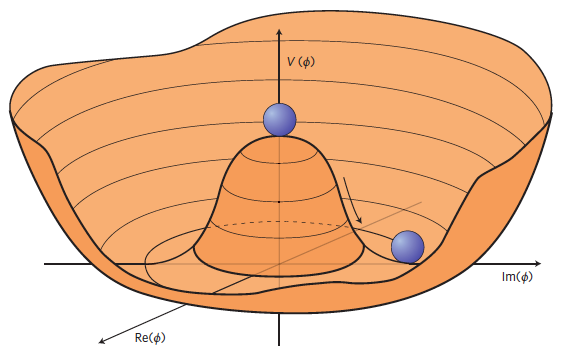
\includegraphics[width=\linewidth,height=\textheight,keepaspectratio]{theory/higgspotential}
        \caption{A two-dimensional representation of the Higgs Potential for a complex Higgs field\cite{higgspotential}.
            Like a ball on a narrow hill, the Higgs field will inevitably roll off to the side into valley below.
            From the Higgs's new perspective at the bottom of this valley,
                the potential no longer appears symmetric,
                leading to the Higgs field acquiring a mass term.
        }
        \label{fig:higgs_potential}
    \end{figure}

    Now for the complications.
    The added symmetries require that the derivative be changed to a covariant derivative 
        $D_{\mu} = \partial_{\mu} - \frac{ig}{2} \wField^a_{\mu} \sigma^a - \frac{ig'}{2} B_{\mu}$.
    Here, $\wField^a_\mu$ and $B_\mu$ correspond to the unbroken $SU(2)$ and $U(1)$ gauge fields respectively.
    This produces a Lagrangian:
    \begin{equation} \begin{split}
        \Lag &= \frac{1}{2} |D_{\mu} \vec{\phi}|^2 +
            \mu^2 \vec{\phi}^\dag \vec{\phi} - \lambda \left( \vec{\phi}^\dag\vec{\phi} \right)^2
        \,.
    \end{split} \end{equation}


    Once again, I allow the scalar field to fall into its offset minimum $v$
        (hereafter referred to as the ``Vacuum Expectation Value'' or \textit{vev})
    \begin{equation}
        v \equiv \frac{\mu}{\sqrt{\lambda}} \textrm{ ,  for   }
            \vec{\phi}(x) \to \vec{h}(x) + \vec{v} = 
            \frac{1}{\sqrt{2}}\minimatrix{0\\h(x)} + \frac{1}{\sqrt{2}}\minimatrix{0\\v} = \frac{1}{\sqrt{2}}\minimatrix{0\\h(x)+v}
        \,.
    \end{equation}
    Worth mentioning is that due to the added groups, there are no longer only two minima.
    Instead, there is now a continuum of equal-valued minima centered on a spherical ``valley'' a distance $v$ from $\phi=0$.
    Substituting into the Lagrangian now produces a more complex expression:
    \begin{equation} \begin{split}
        \label{eq:fullHiggs}
        \Lag & = \frac{1}{2} \left|D_{\mu} \frac{1}{\sqrt{2}}\minimatrix{0\\h(x)+v}\right|^2
            + \mu^2 \left|\frac{1}{\sqrt{2}}\minimatrix{0\\h(x)+v}\right|^2
            - \lambda \left|\frac{1}{\sqrt{2}}\minimatrix{0\\h(x)+v}\right|^4 \\
         & = \Lag_h + \Lag_v
        \,.
    \end{split} \end{equation}
    where $\Lag_h$ takes a form similar to Eqn. \ref{eq:basic_higgs}, incorporating both the $h$ and $h$/$v$ cross terms.
    Meanwhile, $\Lag_v$ refers only to the terms arising from $D_{\mu}$ acting on the vev:
    \begin{equation}
        \label{eq:lagv}
        \Lag_v = \frac{1}{2} (D_{\mu} \vec{v})^2
        \,.
    \end{equation}
    The expansion of this term specifically will lead to the breakdown of Electro-Weak Symmetry,
        and the $W$ and $Z$ bosons acquiring mass.

    %Get covariant derivative, evaluate at vev, pull out W,Z, and photon fields, and their masses (pg 722);
    Expanding only $D_{\mu} \vec{v}$ initially, the $\partial_{\mu}$ immediately vanishes ($v$ is a constant), yielding 
    \begin{equation} \begin{split}
        D^{\mu} v  = \big( \partial^{\mu} & - \frac{ig}{2} \wField^a_{\mu} \sigma^a - \frac{ig'}{2} B_{\mu} \big) \frac{1}{\sqrt{2}}\minimatrix{0\\v} \\
        = \big( & - \frac{ig}{2} \wField^a_{\mu} \sigma^a - \frac{ig'}{2} B_{\mu} \big) \frac{1}{\sqrt{2}}\minimatrix{0\\v} \\
        = - \frac{i}{2} \big( & g \wField^a_{\mu} \sigma^a + g' B_{\mu} \big) \frac{1}{\sqrt{2}}\minimatrix{0\\1} v
        \,.
    \end{split} \end{equation}

    It is useful here to fully expand the $U(1) \times SU(2)$ fields into their matrix components and add them explicitly,
        as doing so reveals the origin of the photon and W and Z bosons.
    \begin{equation} \begin{split}
        g \wField^a_{\mu} \sigma^a + g' B_{\mu} & =
            g \wField^1_{\mu} \sigma^1
            + g \wField^2_{\mu} \sigma^2
            + g \wField^3_{\mu} \sigma^3
            + g' B_{\mu} I \\
        & = \begin{pmatrix}
            0 & g\wField^1_{\mu} \\ g\wField^1_{\mu} & 0 \end{pmatrix}
            + \begin{pmatrix} 0 & -ig\wField^2_{\mu} \\ ig\wField^2_{\mu} & 0 \end{pmatrix}
            + \begin{pmatrix} g\wField^3_{\mu} & 0 \\ 0 & -g\wField^3_{\mu} \end{pmatrix}
            + \begin{pmatrix} g'B_{\mu} & 0 \\ 0 & g'B_{\mu}
        \end{pmatrix} \\
        & = \begin{pmatrix} 
            g\wField^3_{\mu} + g'B_{\mu} & g\wField^1_{\mu} - ig\wField^2_{\mu} \\
            g\wField^1_{\mu} + ig\wField^2_{\mu} & -g\wField^3_{\mu} + g'B_{\mu}
        \end{pmatrix}
        \,.
    \end{split} \end{equation}

    The four components of this matrix will ultimately be associated with the 
        gauge boson fields of the electromagnetic ($A$) and weak ($W$ \& $Z$) interactions
    \begin{equation} \begin{split}
        \label{eq:electroweak_matrix}
        \begin{pmatrix} 
            g\wField^3_{\mu} + g'B_{\mu} & g\wField^1_{\mu} - ig\wField^2_{\mu} \\
            g\wField^1_{\mu} + ig\wField^2_{\mu} & -g\wField^3_{\mu} + g'B_{\mu}
        \end{pmatrix} =
        \begin{pmatrix} 
            \sqrt{g^2 + g^{\prime 2}}\ A_{\mu} & g \sqrt{2}\ W^+_{\mu} \\
            g \sqrt{2}\ W^-_{\mu} & - \sqrt{g^2 + g^{\prime 2}}\ Z^0_{\mu}
        \end{pmatrix}
        \,,
    \end{split} \end{equation}
    with $A$, $W^+$, $W^-$, and $Z^0$ related to the unbroken $\wField^a$ and $B$ fields by
    \begin{equation} \begin{split}
        A_{\mu} & = \frac{1}{\sqrt{g^2 + g^{\prime 2}}} ( g\wField^3_{\mu} + g'B_{\mu} ) \\
        Z^0_{\mu} & = \frac{1}{\sqrt{g^2 + g^{\prime 2}}} ( g\wField^3_{\mu} - g'B_{\mu} ) \\
        W^{\pm}_{\mu} & = \frac{1}{\sqrt{2}} (\wField^1_{\mu} \mp i\wField^2_{\mu})
        \,.
    \end{split} \end{equation}
    The $\sqrt{g^2 + g^{\prime 2}}$ factor is the result of converting between
        $\tinymatrix{Z^0 \\ A}$ and $\tinymatrix{\wField^3 \\ B}$ by way of a rotation matrix
    \begin{equation} \begin{split}
        \begin{pmatrix} Z^0 \\ A \end{pmatrix} =
        \begin{pmatrix}
            \frac{g}{\sqrt{g^2 + g^{\prime 2}}} & \frac{-g'}{\sqrt{g^2 + g^{\prime 2}}} \\
            \frac{g'}{\sqrt{g^2 + g^{\prime 2}}} & \frac{g}{\sqrt{g^2 + g^{\prime 2}}}
        \end{pmatrix} \begin{pmatrix} \wField^3 \\ B \end{pmatrix} = 
        \begin{pmatrix}
            \cos\theta_w & -\sin\theta_w \\
            \sin\theta_w & \cos\theta_w
        \end{pmatrix} \begin{pmatrix} \wField^3 \\ B \end{pmatrix}
        \,,
    \end{split} \end{equation}
    where $\theta_w \equiv \cot(\frac{g'}{g})$ is known as the \textit{weak mixing angle} (AKA the Weinberg angle).

    Returning finally to Eqn. \ref{eq:lagv}, I now have
    \begin{equation} \begin{split}
        \label{eq:lagv_full}
        \Lag_v & = \frac{1}{2} (D_{\mu}^{ij} v_j)^2 \\
        & = \frac{1}{2}
            \frac{1}{\sqrt{2}} \begin{pmatrix} 0 & v \end{pmatrix}
            \left| -\frac{i}{2}
                \begin{pmatrix} 
                    \sqrt{g^2 + g^{\prime 2}}\ A_{\mu} & g \sqrt{2}\ W^+_{\mu} \\
                    g \sqrt{2}\ W^-_{\mu} & - \sqrt{g^2 + g^{\prime 2}}\ Z^0_{\mu}
                \end{pmatrix}
            \right|^2
            \frac{1}{\sqrt{2}} \begin{pmatrix} 0 \\ v \end{pmatrix} \\
        & = \frac{1}{2} \frac{v^2}{2} \frac{1}{4}
            \begin{pmatrix} 0 & 1 \end{pmatrix}
            \begin{pmatrix} 
                \sqrt{g^2 + g^{\prime 2}}\ A_{\mu} & g \sqrt{2}\ W^+_{\mu} \\
                g \sqrt{2}\ W^-_{\mu} & - \sqrt{g^2 + g^{\prime 2}}\ Z^0_{\mu}
            \end{pmatrix}
            \begin{pmatrix} 
                \sqrt{g^2 + g^{\prime 2}}\ A_{\mu} & g \sqrt{2}\ W^+_{\mu} \\
                g \sqrt{2}\ W^-_{\mu} & - \sqrt{g^2 + g^{\prime 2}}\ Z^0_{\mu}
            \end{pmatrix}
            \begin{pmatrix} 0 \\ 1 \end{pmatrix} \\
        & = \frac{1}{2} \frac{v^2}{2} \frac{1}{4}
            \begin{pmatrix} 
                g \sqrt{2}\ W^-_{\mu} & - \sqrt{g^2 + g^{\prime 2}}\ Z^0_{\mu}
            \end{pmatrix}
            \begin{pmatrix} 
                 g \sqrt{2}\ W^+_{\mu} \\
                 - \sqrt{g^2 + g^{\prime 2}}\ Z^0_{\mu}
            \end{pmatrix} \\
        & = \frac{1}{2} \frac{v^2}{2} \frac{1}{4} 
            \left[ 2 g^2  W^-_{\mu} W^+_{\mu}
            + \left(\sqrt{g^2 + g^{\prime 2}}\right)^2 (Z^0_{\mu})^2 \right] \\
        & = \frac{1}{2} \left[ \left(\frac{vg}{2}\right)^2\  W^-_{\mu} W^+_{\mu}
            + \frac{1}{2} \left(\frac{v}{2}\sqrt{g^2 + g^{\prime 2}}\right)^2\ (Z^0_{\mu})^2 \right] \\
        & = \frac{1}{2} \left[ m_W^2 W^{-\ \mu} W^+_{\mu} + \frac{m_Z^2}{2} (Z^0_{\mu})^2 \right]
        \,.
    \end{split} \end{equation}

    As in Section \ref{sec:higgs_mechanism}, the $W$ and $Z$ fields now have additional mass terms associated with their kinetic energy terms,
        with $m_W = \frac{vg}{2}$ and $m_Z = \left(\frac{v}{2}\sqrt{g^2 + g^{\prime 2}}\right) $.
    The photon field $A_{\mu}$ is notably absent in the final Lagrangian, and thus remains massless.
    A similar procedure can then be followed to allow the Higgs Field to interact with fermions
        (albeit with complications arising from mass-mixing and chirality),
        which will grant mass to the Dirac fields.


    % Fermion time!!
%\subsection{Giving Mass to Fermions}
% Ok this is seriously just the same thing but now we have to split the fermion fields into left and right and up-type and down-type
% and split the higgs into the higgs and conjugate higgs and also insert the complex mass matrix except don't insert it for charged leptons
% because reasons or something. And then poof your charged leptons have mass and your quarks have mass and flavour changing

    %Split fermions between right and left fields, assign LH to SU(2) doublets (T=+-1?), RH to SU(2) singlet (T=0), assign Y too (pg724-725);
    %Sandwitch covariant derivative terms between fermion fields, expand to get field currents (pg 725-726);
    %*Try* to expand masses and fail because of representation incompatibilities (pg 725);
    %Anamoly cancellation thing I'll probably ignore (pg 726);
    %Add higgs interaction psibar phi psi to fermion lagrangian, expand into higgs interaction, convert to fermion mass (pg 734);

%Further work must then be done to couple the higgs boson to fermions and itself
%You need to tie k2v, kl, and kv in to the shape of the higgs potential here
\section{Keystone of the Standard Model: The Higgs Boson} \label{sec:higgs_boson}

    With the critical role of the Higgs Field established, it is now time to return to Eqn. \ref{eq:fullHiggs}
        and investigate $\Lag_h$, the Lagrangian of the Higgs boson itself.
    The terms involved therein provide information not only about the Higgs Field,
        but also provide insight into how the Higgs may be further studied:
    \begin{equation} \begin{split}
        \Lag &= \frac{1}{2} |D_{\mu} \vec{\phi}|^2 +
            \mu^2 \vec{\phi}^\dag \vec{\phi} - \lambda \left( \vec{\phi}^\dag\vec{\phi} \right)^2
        \\&= \Lag_K + \Lag_U \quad ; \quad 
            \Lag_K \equiv \frac{1}{2} |D_{\mu} \vec{\phi}|^2 \quad , \quad
            \Lag_U \equiv \mu^2 \vec{\phi}^\dag \vec{\phi} - \lambda \left( \vec{\phi}^\dag\vec{\phi} \right)^2
        \,.
    \end{split} \end{equation}
    
    To make expansion easier, I will expand the covariant derivative terms ($\Lag_K$) first
        and then add the expanded $\Lag_U$ terms.
    Starting with $\Lag_K$, (and defining $Q_{\mu}$ as the matrix from Eqn. \ref{eq:electroweak_matrix})
    \begin{equation} \begin{split}
        \Lag_K &= \frac{1}{2} |D_{\mu} \vec{\phi}|^2
            \\&= \frac{1}{2} (D^{\mu} \vec{\phi})^\dag (D_{\mu} \vec{\phi})
                = \frac{1}{2} \left[(\partial^{\mu} - \frac{i}{2}Q^{\mu}) \vec{\phi}\right]^\dag
                \left[(\partial_{\mu} - \frac{i}{2}Q^{\mu}) \vec{\phi}\right]
            \\&= \frac{1}{2} \left(\vec{\phi}^\dag \partial^{\mu} + \frac{i}{2} \vec{\phi}^\dag Q^{\mu \dag} \right)
                \left(\partial_{\mu}\vec{\phi} - \frac{i}{2}Q_{\mu}\vec{\phi} \right)
            \\&= \frac{1}{2} \left(
                \vec{\phi}^\dag \partial^{\mu} \partial_{\mu}\vec{\phi}
                - \frac{i}{2} \vec{\phi}^\dag \partial^{\mu} Q_{\mu}\vec{\phi}
                + \frac{i}{2} \vec{\phi}^\dag Q^{\mu \dag} \partial_{\mu}\vec{\phi}
                + \frac{1}{4} \vec{\phi}^\dag Q^{\mu \dag} Q_{\mu}\vec{\phi}
                \right)
            \\&= \frac{1}{2} \left(
                | \partial_{\mu}\vec{\phi} |^2
                + \frac{1}{4} \vec{\phi}^\dag Q^{\mu} Q_{\mu} \vec{\phi}
                \right)
                = \frac{1}{2} | \partial_{\mu}h |^2 + \frac{1}{8} \vec{\phi}^\dag Q^{\mu}Q_{\mu} \vec{\phi}
            \\&= \frac{1}{2} | \partial_{\mu}\vec{\phi} |^2 + \frac{1}{8} 
                    \frac{1}{\sqrt{2}}\minimatrix{0 & h^* + v} Q^{\mu}
                    Q_{\mu} \frac{1}{\sqrt{2}}\minimatrix{0 \\ h + v}
            \\&= \frac{1}{2} | \partial_{\mu}h |^2
                + \frac{1}{2} \frac{1}{8} \frac{v^2}{v^2} \left[ 2 g^2  W^-_{\mu} W^+_{\mu}
                + \left(\sqrt{g^2 + g^{\prime 2}}\right)^2 (Z^0_{\mu})^2 \right] (h+v)^2
        \,.
    \end{split} \end{equation}

    The $(h+v)^2$ term will produce couplings quadratic in $v$ ($\Lag_v$ of Eqn. \ref{eq:lagv_full}), and both linear and quadratic in $h$.
    Replacing the coefficients in front of the $W$ and $Z$ fields with their respective masses
        and expanding these terms out (except the quadratic $v$ term, $\Lag_v$) yields
    \begin{equation} \begin{split}
        \Lag_K &= \frac{1}{2} | \partial_{\mu}h |^2
                + \frac{1}{2v^2} \left[ m_W^2\  W^{-\ \mu} W^+_{\mu}
                + \frac{1}{2} m_Z^2\ (Z^0_{\mu})^2 \right] (h+v)^2 \\
        &= \frac{1}{2} | \partial_{\mu}h |^2
            + \frac{1}{v}\left[ m_W^2 W^{-\ \mu} W^+_{\mu} + \frac{m_Z^2}{2} (Z^0_{\mu})^2 \right] h
            + \frac{1}{2v^2} \left[ m_W^2 W^{-\ \mu} W^+_{\mu} + \frac{m_Z^2}{2} (Z^0_{\mu})^2 \right] h^2
            + \Lag_v % FIXME: I'm missing a factor of 2 here :-/
        \,.
    \end{split} \end{equation}

    Often, $W$ and $Z$ field interactions are considered for the same process,
        and as such are described together simply as vector bosons, $V$:
    \begin{equation} \begin{split}
        \Lag_K = \frac{1}{2} | \partial_{\mu}h |^2 + \Lag_v
            + \frac{1}{v} m_V^2 V^2 h + \frac{1}{2v^2} m_V^2 V^2 h^2
        \,.
    \end{split} \end{equation}

    \noindent Returning to $\Lag_U$ and substituting in for $v$
    \begin{equation} \begin{split}
        \Lag_U &= \mu^2 \vec{\phi}^\dag \vec{\phi} - \lambda \left( \vec{\phi}^\dag\vec{\phi} \right)^2
        \\&= - \mu^2 h^2 -\lambda v h^3 - \frac{1}{4} \lambda h^4
        \\&= - \mu^2 h^2 - \mu \sqrt\lambda h^3 - \frac{1}{4} \lambda h^4
        \,.
    \end{split} \end{equation}
    Identifying the Higgs mass $m_h$ as $\sqrt{2}\mu$,
        and the vev $v$ as $\frac{\mu}{\sqrt{\lambda}} = \frac{m_h}{\sqrt{2 \lambda}}$,
        I can now write the full Lagrangian for the Higgs field\cite{Halzen_book}
    \begin{equation} \begin{split} \label{eq:higgsfull}
        \Lag_h &= \Lag_K + \Lag_U
        \\&= \left[ \frac{1}{2} | \partial_{\mu}h |^2
                + \frac{1}{v} m_V^2 V^2 h + \frac{1}{2v^2} m_V^2 V^2 h^2
            \right]
            + \left[ - \frac{1}{2} m^2_h h^2 - m_h \sqrt{\frac{\lambda}{2}} h^3 - \frac{1}{4} \lambda h^4 \right]
        \\&= \frac{1}{2} \left(\partial^2 - m_h^2 \right) h^2
            + \sqrt{2\lambda} \frac{m_V^2}{m_h} V^2 h + \lambda \frac{m_V^2}{m_h^2} V^2 h^2
            - m_h \sqrt{\frac{\lambda}{2}} h^3 - \frac{1}{4} \lambda h^4
        \\&= \frac{1}{2} \left(\partial^2 - m_h^2 \right) h^2
            + g_{HVV} V^2 h + \frac{g_{HHVV}}{2} V^2 h^2
            + \frac{g_{HHH}}{3!} h^3 + \frac{g_{HHHH}}{4!} h^4 \\
        \,.
    \end{split} \end{equation}
    where the coupling terms are defined as
    \begin{equation} \begin{split} \label{eq:higgscouplings}
        g_{HVV}  \equiv 2\sqrt{2\lambda} \frac{m_V^2}{m_h} ,\;
        g_{HHVV} \equiv 4\lambda \frac{m_V^2}{m_h^2} ,\;
        g_{HHH}  \equiv 3\sqrt{2\lambda} m_h ,\;
        g_{HHHH} \equiv 6 \lambda
    \end{split} \end{equation}
    The first term of this Lagrangian is simply the kinetic energy term for the Higgs.
    The remaining terms correspond, respectively,
        to the Higgs/vector boson interaction $g_{HVV}$,
        Higgs/vector boson four-point interaction $g_{HHVV}$,
        Higgs self-coupling $g_{HHH}$,
        and finally the Higgs four-point self-coupling $g_{HHHH}$.

    In 2012, the Higgs boson was detected with a mass of 125 GeV, solidifying both its existence and crucial role in the Standard Model.
    More to the point, its detection confirmed the existence of the Higgs kinetic energy term in the Lagrangian,
        along with its coupling terms to fermions and vector bosons.
    The various self-interaction terms however, are still on more tenuous grounds.
    If they exist at all, there is no guarantee that these interactions have the coupling strength indicated by Eqn. \ref{eq:higgsfull}.
    In order to account for this uncertainty, the Lagrangian can be rewritten with arbitrary scaling factors for the interaction couplings
    \begin{equation} \begin{split} \label{eq:higgskappas}
        \Lag_h &= \frac{1}{2} \left(\partial^2 - m_h^2 \right) h^2
            + \kv g_{HVV} V^2 h + \kvv \frac{g_{HHVV}}{2} V^2 h^2
            + \kl \frac{g_{HHH}}{3!} h^3 + \kappa_{2\lambda} \frac{g_{HHHH}}{4!} h^4
        \,.
    \end{split} \end{equation}

    The new $\kappa$ terms are ratios of the coupling, as predicted by the Standard Model ($g$), to the true coupling value ($g'$).
    The new $\kappa$ terms are ratios of the true coupling value ($g'$)
        to the coupling as predicted by the Standard Model ($g$).
    For example, $\kappa_V \equiv \frac{g'_{HVV}}{g_{HVV}}$.
    A $\kappa$ value of 1 indicates consistency with the coupling strength predicted by the Standard Model.
    Any value other than 1 would indicate deviation from the Standard Model,
        which would need to be explained with a modification to the (or entirely new) theory.
    As of 2020, $\kv$ has been measured at a value of $1.05 \pm 0.04$,
        based on combined analysis of single Higgs production processes\cite{paper:higgs_combined}.
    The couplings $\kvv$, $\kl$, and $\kappa_{2\lambda}$ however, do not significantly affect the production of single Higgs processes.
    The quartic coupling $\kappa_{2\lambda}$ is outside the scope of this thesis,
        but $\kvv$ and $\kl$ can be measured through their effect on di-Higgs production.
    Constraining the range of these values could yield key insight into the validity of the Standard Model and the nature of the Higgs Potential,
        and will therefore be the target of this thesis.


%How do we test any of this?
%From Lagrangian to Cross-Section:
%    I need to study up on exactly how you go from the lagrangian to the Feynman rules, and from there to a calcualable cross section
\section{From Theory to Experiment: The Feynman Rules and Cross-Sections} \label{sec:feyn_rules}
    
    %Justify why we care about cross sections
    After so much discussion of theory, the obvious question to ask is: how can this be tested?
    The most direct physically observable effects of the equations of the Standard Model are those of \textit{differential cross-sections}.
    Cross-sections will be discussed in more detail in Section \ref{sec:lhc-interaction_region},
        but for now it is sufficient to state that the probability of some physical interaction taking place
        is directly proportional to its differential cross-section.
    Here I will provide a general outline for how the Lagrangian of Eqn. \ref{eq:higgskappas} can be related to a measurable cross-section.

    In quantum mechanics, probabilities are defined as the absolute square of amplitudes of wave functions, $\left|\braket{\psi}\right|^2$.
    The probability of a transition between different states of a wavefunction are similarly represented
        as the absolute square of the original state, $\psi_i$, \textit{in the basis of} the final state $\psi_f$,
        written $ |\Tbraket{\psi_f}{\psi_i}|^2$.
    In Quantum Field Theory, states correspond to which particles are in existence at a given moment.
    Thus, a state of one electron and one anti-electron could be written as $\ket{e \bar{e}}$,
        and the transition of an electron-positron pair into a muon/anti-muon pair could be written
        as $\Tbraket{\mu \bar{\mu}}{e \bar{e}}$.

    The process used in this thesis to probe the Higgs's $\kappa$ values is that of
        Vector Boson Fusion (VBF) to a di-Higgs pair decaying to 4b (\vbfhhproc).
    That is, two incoming quarks, $\ket{q_1 q_2}$, form the initial state of this process.
    These quarks each emit a vector boson (either $W^{\pm}$ or $Z^0$), 
        which will in turn fuse into an intermediate state of two Higgs Bosons.
    After being deflected by the weak boson ejection, the quarks then continue on,
        possibly having been flavor-changed if they emitted a charged $W$.
    Meanwhile, the Higgs bosons have a very short lifetime and will decay almost immediately into one of a number of possible particles.
    The likelihood that the Higgs will decay into a given state is given by that state's \textit{branching ratio}.
    As seen from Table \ref{tab:higgsbranching}, a bottom/anti-bottom quark pair is the most likely decay product of the Higgs,
        hence its use as the final state in this analysis.
    The final state of this process consists of two Higgs and the $b \bar{b}$ pairs.
    However, since the Higgs' coupling to the bottom quark does not probe the couplings of interest in this thesis,
        for this chapter I want to focus only on the intermediate state
        consisting of two Higgs and two deflected quarks,
            $\bra{h_1 h_2 q_3 q_4}$.
    I can then write the transition of this process as $\Tbraket{ h_1 h_2 q_3 q_4}{q_1 q_2}$.
    %It should be noted that while there are other intermediate processes besides VBF
    %    that could produce these same initial and final states, 
    %    but these will not be considered in this analysis.

    \begin{table}[tbh]
\begin{center}
\caption{
    Branching ratio of the Higgs to its most common final states.
    The $b \bar{b}$ final state is dominant with over twice the branching ratio of the subleading decay mode,
        and nearly an order of magnitude higher than the sub-sub-leading decay mode\cite{particlephysicsreview2021}.
}
\label{tab:higgsbranching}
%\footnotesize
\begin{tabular}{|l|l|l|}
    \toprule
    Decay channel & Branching ratio & Rel. uncertainty  \\
    \midrule
    $ H \to b \bar{b}        $    & $5.82 \times 10^{-1} $    & $ +1.2\% \atop -1.3\% $ \\
    $ H \to W^+ W^-          $    & $2.14 \times 10^{-1} $    & $\pm 1.5\%        $   \\
    $ H \to \tau^+ \tau^-    $    & $6.27 \times 10^{-2} $    & $\pm 1.6\%        $   \\
    $ H \to c \bar{c}        $    & $2.89 \times 10^{-2} $    & $ +5.5\% \atop -2.0\% $ \\
    $ H \to ZZ               $    & $2.62 \times 10^{-2} $    & $\pm 1.5\%        $   \\
    $ H \to \gamma \gamma    $    & $2.27 \times 10^{-3} $    & $    2.1\%        $   \\
    $ H \to Z \gamma         $    & $1.53 \times 10^{-3} $    & $\pm 5.8\%        $  \\
    $ H \to \mu^+ \mu^-      $    & $2.18 \times 10^{-4} $    & $\pm 1.7\%        $  \\
    \bottomrule
\end{tabular}
\end{center}
\end{table}


    In principle, this transition process can take a finite period of time.
    In the realm of high energy physics experiments though,
        the interacting particles are moving so fast that the interaction period can be thought of as occurring at a single instant in time.
    Given this context, the initial state occurs in the (comparatively) distant past, $t_i$, and the final state in the equally distant future, $t_f$.
    Since the transition occurs at an instantaneous moment,
        I need to perform a time-translation transformation on both states to place them at the moment of the transition, $t_0$.
    Using the Hamiltonian $H \equiv i\partial_0$ as the time translation operator,
        I can relate the initial state at $t_0$ to its time $\Delta t$ units in the future, $t_i$, by the transformation
    \begin{equation}
        \ket{q_{1} q_{2} (t_i)} = e^{i\Delta tH}\ket{q_{1} q_{2} (t_0)}
        \,.
    \end{equation}
    The same can be done to transform the final state backwards in time
    \begin{equation}
        \bra{h_1 h_2 q_{3} q_{4} (t_f)}
        = \bra{h_1 h_2 q_{3} q_{4} (t_0)} (e^{i(-\Delta t)H})^\dag
        = \bra{h_1 h_2 q_{3} q_{4} (t_0)} e^{i\Delta tH}
        \,.
    \end{equation}
    Putting both of these together yields
    \begin{equation} \begin{split} \label{eq:transition_amplitude}
        \Tbraket{ h_1 h_2 q_{3} q_{4} (t_f)}{q_{1} q_{2} (t_i)}
        &= \TbraketA{ h_1 h_2 q_{3} q_{4} (t_0)}{e^{i\Delta tH} e^{i\Delta tH}}{q_{1} q_{2} (t_0)}
        \\&= \TbraketA{ h_1 h_2 q_{3} q_{4} (t_0)}{e^{2\Delta tH}}{q_{1} q_{2} (t_0)}
        \\&= \TbraketA{ h_1 h_2 q_{3} q_{4} (t_0)}{1 + iT}{q_{1} q_{2} (t_0)}
        \,.
    \end{split} \end{equation}

    In the last step, the exponential operator is expanded as an infinite series of terms,
        in a reversal of the procedure from Section \ref{sec:group_theory}.
    The first of these terms will just be 1, corresponding to the static situation in which no interaction occurs at all.
    The sum of the remaining terms, represented as $iT$, is the part relevant for calculating the interaction probability,
        with the entire transition amplitude referred to as the \textit{invariant amplitude}, $\invAmp$:
    \begin{equation}
        i\invAmp \equiv \TbraketA{ h_1 h_2 q_{3} q_{4} (t_0)}{iT}{q_{1} q_{2} (t_0)}
        \,.
    \end{equation}

    As stated above, the differential cross-section, $\dXsec$,
        of a process is proportional to its probability $\mathcal{P}$,
        which in turn can be related to the invariant amplitude
    \begin{equation} \begin{split}
        \dXsec &\propto \mathcal{P}( q_{1} q_{2} \rightarrow q_{3} q_{4} h_1 h_2 ) 
            = \left| \TbraketA{ h_1 h_2 q_{3} q_{4} (t_0)}{iT}{q_{1} q_{2} (t_0)} \right|^2 
            = |i \invAmp|^2 
        \\\dXsec &= \Gamma(p_1, p_2, ...) |\invAmp|^2
        \,.
    \end{split} \end{equation}

    Where $\Gamma(p_1, p_2, ...)$ is a function of the scattering kinematics,
        e.g.\ the particles' crossing angle, energies, and momenta, etc.
    These kinematics are mostly related to the properties of the setup of the scattering experiment under consideration.
    All dependence on the Standard Model Lagrangian is contained within the $\invAmp$ term,
        and the remainder of this chapter will be devoted to its calculation.
    To do this, I turn to Feynman diagrams.

    Calculation of the transition expectation value of the $iT$ term has historically been a very technical challenge.
    Feynman diagrams are an elegant tool for performing this task more easily and intuitively.
    The general process to using them begins with the following steps:
    \begin{itemize}
        \item Draw the initial and final states of the process in question as dots
        \item Fully connect the initial and final state particles using any \textit{valid} intermediate lines and vertices
        \item Valid connections can be identified through the terms present in the Lagrangian:
        \begin{itemize}
            \item Kinetic energy terms correspond to lines connecting a particle to itself
            \item Interaction terms correspond to interaction vertices, connecting three or more particles at a time
            \item All vertices must ensure conservation of any relevant quantum number
        \end{itemize}
        \item Repeat the above steps in order to draw all possible diagrams
    \end{itemize}

    This final step may seem impossible, given that an infinite number of intermediate particles can be inserted between any two states.
    Recall from the structure of $\invAmp$, that $iT$ is not one term, but in fact an infinite series expansion of the Hamiltonian operator.
    For most situations, each higher order of the terms will contribute less to the overall calculation.
    Eventually, the higher-order terms will contribute so little that they can be safely ignored.
    This property is directly reflected in the Feynman Diagrams, in the form of \textit{loops}.
    Any loop in a diagram indicates that the diagram is a higher order term of the expansion.
    A diagram with no loops -- referred as ``tree-level'' or ``leading order'' (LO) -- is part of the first term of $iT$.
    Diagrams with one loop are part of the second term (next-to-leading order, or NLO),
        two loops the third (next-to-next-to-leading order, or NNLO), and so forth.

    One need only draw as many diagrams as is needed for the level of desired precision.
    As a side note, just as successive loops correspond to higher order terms in $iT$,
        diagrams which are not fully connected correspond to the ``1'' term from the original $1+iT$ in Eqn. \ref{eq:transition_amplitude},
        hence why disconnected diagrams are ignored entirely.

    \begin{figure}
    \centering
    \begin{subfigure}{0.32\textwidth} 
        \resizebox{0.9\textwidth}{!}{
\begin{tikzpicture} \begin{feynman}
    \vertex (kv1) {$\kv$};
    \vertex [below=of kv1] (kv2) {$\kv$};
    \vertex [right=of kv1] (h1) {$h_1$};
    \vertex [right=of kv2] (h2) {$h_2$};
    \vertex [above left=of kv1] (vb1);
    \vertex [below left=of kv2] (vb2);
    \vertex [left=of vb1] (q1) {$q_{1}$};
    \vertex [left=of vb2] (q2) {$q_{2}$};

    \vertex [above=of h1] (q3) {$q_{3}$};
    \vertex [below=of h2] (q4) {$q_{4}$};

    \diagram* {
        (q1) -- (vb1) -- (q3),
        (q2) -- (vb2) -- (q4), 
        (vb1) -- [boson] (kv1) -- [boson] (kv2)-- [boson] (vb2),
        (h1) -- [scalar] (kv1),
        (h2) -- [scalar] (kv2),
    };
\end{feynman} \end{tikzpicture}
}
 
        \caption{$M_t$}
        \label{fig:tree_level_vbfhh:kv}
    \end{subfigure}
    \begin{subfigure}{0.32\textwidth}
        \begin{tikzpicture} \begin{feynman}
    \vertex (kv) {$\kv$};
    \vertex [right=of kv] (kl) {$\kl$};
    \vertex [above right=of kl] (h1) {$h_1$};
    \vertex [below right=of kl] (h2) {$h_2$};
    \vertex [above left=of kv] (vb1);
    \vertex [below left=of kv] (vb2);
    \vertex [left=of vb1] (q1i) {$q_{i1}$};
    \vertex [left=of vb2] (q2i) {$q_{i2}$};

    \vertex [above=of h1] (q1f) {$q_{f1}$};
    \vertex [below=of h2] (q2f) {$q_{f2}$};

    \diagram* {
        (q1i) -- (vb1) -- (q1f),
        (q2i) -- (vb2) -- (q2f), 
        (vb1) -- [boson] (kv) -- [boson] (vb2),
        (kv) -- [scalar] (kl),
        (h1) -- [scalar] (kl) -- [scalar] (h2),
    };
\end{feynman} \end{tikzpicture}
 
        \caption{$M_s$}
        \label{fig:tree_level_vbfhh:kl}
    \end{subfigure}
    \begin{subfigure}{0.32\textwidth}
        \resizebox{0.8\textwidth}{!}{
\begin{tikzpicture} \begin{feynman}
    \vertex (k2v) {$\kvv$};
    \vertex [above right=of k2v] (h1) {$h_1$};
    \vertex [below right=of k2v] (h2) {$h_2$};
    \vertex [above left=of k2v] (vb1);
    \vertex [below left=of k2v] (vb2);
    \vertex [left=of vb1] (q1i) {$q_{i1}$};
    \vertex [left=of vb2] (q2i) {$q_{i2}$};

    \vertex [above=of h1] (q1f) {$q_{f1}$};
    \vertex [below=of h2] (q2f) {$q_{f2}$};

    \diagram* {
        (q1i) -- (vb1) -- (q1f),
        (q2i) -- (vb2) -- (q2f), 
        (vb1) -- [boson] (k2v) -- [boson] (vb2),
        (h1) -- [scalar] (k2v) -- [scalar] (h2),
    };
\end{feynman} \end{tikzpicture}
}
 
        \caption{$M_x$}
        \label{fig:tree_level_vbfhh:k2v}
    \end{subfigure}
    \caption{Tree-level diagrams of the \hhproc process.}
    \end{figure}

    Once all possible diagrams have been drawn to the order desired, each diagram has a value assigned to it.
    ``Feynman Rules'' are the rules governing how these values are assigned.
    The rules are derived based on the structure of the Lagrangian and are rather extensive;
        hence, they will not be listed here.
    After the values have been determined, the invariant amplitude is trivially calculated as the sum of the values of all drawn diagrams.
    The \hhproc process studied here is primarily done at tree-level
        (Fig. \ref{fig:tree_level_vbfhh:kv}-\ref{fig:tree_level_vbfhh:k2v}),
        but N\textsuperscript{3}LO calculations are also used to some degree.

    Finally, the differential cross-section can be calculated as the absolute square of the sum of the Feynman Diagrams.
    There is one critical (to this analysis) detail of the Feynman rules I will mention,
        which is that each diagram's value $M$ is proportional to the \textit{product of the coefficients}
        associated with each interaction vertex in the diagram.
    Take for example Fig. \ref{fig:tree_level_vbfhh:kv}, which contains four total vertices;
        two corresponding to the Higgs-Vector Boson interaction (whose coefficient based on Eqn. \ref{eq:higgskappas} is $\kv q_V$),
        and two corresponding to the quark-Vector Boson interaction (whose coefficient is $c_{qV}$).
    As per the Feynman rules, this means that $M_t$ is proportional to $\kv q_V \kv q_V c_{qV} c_{qV}$.
    The quantities I am interested in are of course the $\kappa$ values,
        so I can pull these values out in front of the invariant amplitude as $M_t \rightarrow \kv^2 M_t$.
    At tree-level, I can then write out the absolute square of the invariant amplitude as
    \begin{equation} \begin{split} \label{eq:tree_level_invamp}
        |\invAmp|^2 &= |  \kv^2 M_t + \kv \kl M_s + \kvv M_x |^2
        \\&= \kv^2 \kl^2 M_s^2 + \kv^4 M_t^2 + \kvv^2 M_x^2 
            \\&\qquad + \kv^3 \kl (M_s^* M_t + M_t^* M_s) 
            \\&\qquad + \kv \kl \kvv (M_s^* M_x + M_x^* M_s ) 
            \\&\qquad + \kv^2 \kvv (M_t^* M_x + M_x^* M_t )
        \\\dXsec \propto |\invAmp|^2 &= \kv^2 \kl^2 a_1 + \kv^4 a_2 + \kvv^2 a_3 + \kv^3 \kl a_4 + \kv \kl \kvv a_5 + \kv^2 \kvv a_6
        \,.
    \end{split} \end{equation}

    As noted earlier, the precise value of this cross-section will vary depending on the kinematics of the incoming particles,
        most notably their center of mass (CoM) energy.
    But for this process to occur at all, the CoM energy must be at least the combined mass of the two Higgs Bosons (250 GeV).
    Only a handful of facilities in the world are capable of producing energies at this scale,
        and to produce di-Higgs processes with any appreciable abundance,
        even higher energies are required.
    For measuring the Higgs self-couplings, there is only one machine on the planet that will suffice.

 %TODO

% Ch3: LHC - DRAFT 0
%\chapter{The LHC}\label{chapter:lhc}

% Purpose, obviously -- DONE
The high mass and short life-time of the Higgs Boson ensures that it cannot be readily found in nature.
In order to study the Higgs Boson then, it must first be artificially created through extremely high-energy physical interactions.
The Large Hadron Collider (LHC), among the largest and most complex machines ever constructed, was designed for just such a purpose.
Built by the European Organization for Nuclear Research (CERN, from the French \textit{Conseil Européen pour la Recherche Nucléaire}) with the goal of studying high-energy physics,
the LHC is able to achieve energies well in excess of any previous particle physics experiments.

% Why is 8 and then 13 TeV so critical for Higgs measurement? -- A: because cross section scales with energy, and we just wanted the highest energy possible TODO
% ok wait, I should probably explain what the LHC is even colliding, and why. i.e. how do you generate a "high energy interaction" TODO
% in fact, I kinda need to explain what a "collider" even is. Why are we smashing things together? Maybe it's worth discussing rutherford scattering and the whole "high energy = small wavelength = tinier things you can probe"?

% General history, size, specs TODO
Construction of the LHC took place between 1995 and 2007, over 40 meters underground beneath the French/Swiss border, near Geneva Switzerland. 


how does a particle accelerator make things go fast?
talk about magnets, centripital force, limits to energy based on mag field and radius.
PDF issues of using protons.
Why do we use protons at the LHC?
EM radiation from changing direction, which affects protons less.
Also they're bigger, which is handy (is it?)

run 1/2/3 history discussion.

What does the LHC do, and why?
It's really worth asking why the mechanism of studying fundamental physics is as crude as smashing particles together.
ok but is it though? cross-section of an interaction scales with CoM energy. That's it. Do I really want to be *that* asshole going on about historical bs?


I'm probably going to scrap this whole stupid paragraph and everything it discusses.
Long ago, small things were discovered by looking at them with a microscope.
This meant bouncing light (photons) off things and looking at that reflected light.
At the dawn of atomic physics (1908), Rutherford worked out the structure of the atom by scattering alpha particles off of gold foil.
Later, in 1968, the proton itself was determined to consist of smaller ``partons" based on higher energy scattering experiments performed at SLAC.
The precident set in these, and many other, experiments was that hitting things at higher energy gives a more detailed view of objects.

    


\section{Accelerator Ring}
    Gotta go fast! (Beam injection and main ring specs).
    I'm noticing there isn't much discussion on the actual beam injection, so for now I actually think I might just combine it with the main ring section.

\section{Interaction Region}
    Particles go smash
    - the beampipe focusing magnets,
    - beam crossing point: how do bunches cross each other and interact
    - luminosity: what is it, what determines it 
    - bunch crossing
    - interaction rate: ~1000 particles every 25 ns w/in |eta| < 2.5.


% Ch4: ATLAS - DRAFT 0
%% Structure
%    intro
%    purpose
%    (maybe) helix coords (appendix?)
%    general barrel/endcap cylindrical structure
%    walkthrough of the systems, from inner to outer, discussing why they are there and their basic purpose
%    Then split off into sections for the individual subsystems

    %Discussion of radiation hardness?
    %Things in the endcap suffer from more radiation exposure than things in the barrel
    %    (you should be able to show this from the basic kinematics of the particle beams. most energy is deposited in parallel to the beams, not orthogonal to them)
    %things closer to the IR suffer more than things further away (literally just the inverse-square law)

    %Discussion of using cheaper things as you get further out? (better angular resolution with lower spatial resolution, larger area to be covered, less risk from radiation damage)


\chapter{ATLAS} 
    % Intro
    Production of new physics and particles is of little use without the ability to observe said physics.
    Herein lies the purpose of ATLAS.
    One of the two general purpose detectors at the LHC, construction of the ATLAS detector was completed on October 4, 2008.
    ATLAS is among the largest particle detectors ever built, measuring 46m long with a 25m diameter, and weighing in at 7,000 tonnes \cite{atlas_website}.

    \begin{figure}
        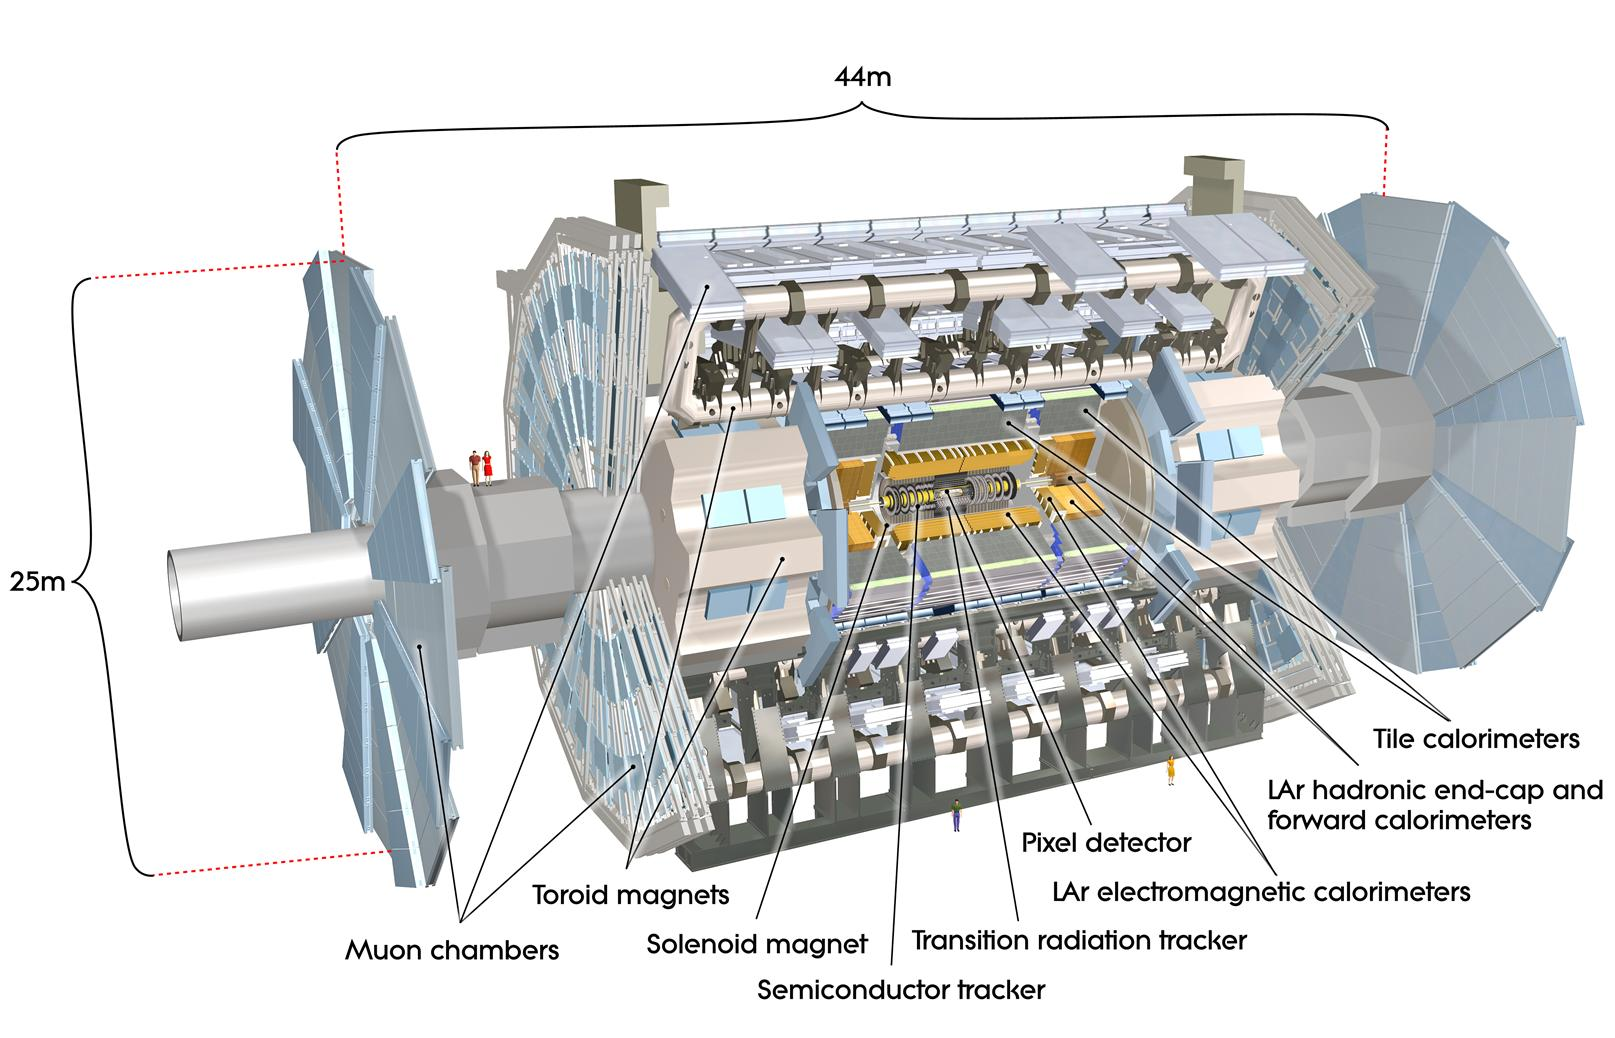
\includegraphics[width=\linewidth,height=\textheight,keepaspectratio]{atlas/atlas_xsec}
        \caption{Cutaway view of the ATLAS detector \cite{Pequenao:1095924}}
        \label{fig:atlas_xsec}
    \end{figure}

    % Purpose
    Core purpose is to accurately record the physical properties of the particle interactions which take place in the interaction region of the detector.
    Most of the particles of interest are extremely short-lived, and so their properties cannot be measured directly.
    Instead, we must detect the decay products of these particles, and reconstruct the original particles of interest after the fact.
    Accurate reconstruction of these original particles is critically dependant on measuring, as precisely as possible, the physical properties of the decay products.
    More specifically, ATLAS is designed to record the paths and decay showers of the particles which pass through the detector, in order to determine their mass, energy, momentum, and electric charge.

    % General barrel/endcap cylindrical structure
    In order to measure all the required properties, ATLAS is divided into many different subsystems.
    Each of these subsystems has a very different design and objective, but they are all constructed with roughly the same overall cylindrical geomtry.
    The reason for this design is simple kinematics.
    The LHC particle beams cross with no initial transverse momentum, which means particles are ejected without preference in the radial angle $\phi$.
    Furthermore, the extremely high longitudinal momentum of the beams results in many particles continuing along a highly "forward" (parallel to the beampipe) trajectory.
    These two properties lead naturally to a radially symmetric detector which is elongated in the forward direction; a cylinder centered on the beam axis.
    To accomodate this geometry, the various sub-detectors of ATLAS are generally split into two distinct parts, called "barrels" and "endcaps".
    The barrels are a series of radially symmetric cylindrical shells, concentric about the beampipes, meant to detect particles moving primarily in the transverse direction.
    Conversely, the endcaps are a series of flat, circular plates, stacked one behind the next along the beampipes, intended to detect more forward particles.

    \begin{figure}
        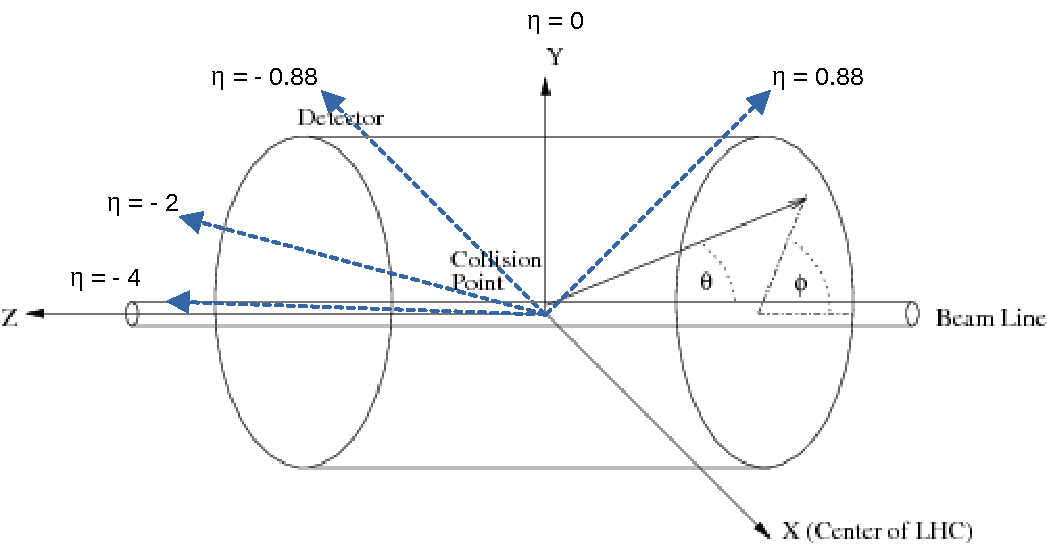
\includegraphics[width=\linewidth,height=\textheight,keepaspectratio]{atlas/atlas_coords}
        \caption{Illustration of the cylindrical coordinate system used in ATLAS \cite{Schott:1699952}}
        \label{fig:atlas_coords}
    \end{figure}

    % Walkthrough of the systems, from inner to outer, discussing why they are there and their basic purpose
    The various detector subsystems can be broken up into three primary groups, based on the subsystems' purpose.
    Moving out from the interaction region, the subsystems can be classified as belonging to the Inner Detector, the Calorimeters, or the Muon Spectrometer.
    The first of these, located as close in $r$ and $z$ as possible, is the Inner Detector system.
    The Inner Detector is desigined to provide momentum measurement, vertexing, and electron identification.
    It must be located so close to the interaction region in order to permit detection of short lived particles like b-quarks and tau leptons \cite{id_tdr}.
    Following immediately behind (endcap) and around (barrel) the Inner Detector is the collection of sensors comprising the Calorimetry system.
    These sensors are purpose-built to measure the energy of incoming particles and also provide supplementary tracking information for particle trajectories.
    Their location between the IR and Muon System is based on the fact that calorimeters function by absorbing all of a particle's energy, thereby stopping them.
    Since their function necessarily stops particles, they must be placed outside the range of the tracking system, as otherwise the trackers would never see particles.
    The Muon system however functions best when only muons traverse it, and so the calorimeters are intentionally placed between the IR and the Muon Spectrometer in order to shield the Muon system from unwanted hadrons.
    Finally, at the outer edge of ATLAS, is the Muon Spectrometer, which has been built to measure the momentum of muons leaving the detector volume.
    


% Then split off into sections for the individual subsystems


\section{Inner Detector} \label{sec:inner_detector}
    % Purpose of subsystem
    % Basic specs
    % What mechanism is used to achieve this purpose
    % What are the individual detectors and how do they contribute to this goal
    
    The Inner Detector system is intended to provide measurement of particles' momentum, provide vertex information, and help in identifying electrons.
    The way it achieves these goals is primarily through a series of very high resolution tracking sensors, which are used to trace out the paths that particles traverse as they leave the IR. 
    Momentum and charge measurement is facilitated by using a solenoid magnet to encompass the entire Inner Detector with a 2T axial magnetic field.
    This field bends the high-momentum charged particles into a helical trajectory, allowing their momentum, mass, and charge to be determined from the shape of the particle's path.
    The entire ID system, consisting of three independent detectors, measures 5.3 m in length and 2.5 m in diameter, and is able to provide accurate tracking within $|\eta| < 2.5$ \cite{id_tdr}.
    From the innermost to outermost, the sub-detectors are the Pixel Detector, the Semiconductor Tracker (SCT), and the Transition Radiation Tracker (TRT).
    The Pixel Detector and SCT together are responsible for high resolution tracking of particle trajectories.
    Further from the IR, the TRT provides more particle tracking capability at lower resolution (but higher statistics), as well the ability to help distinguish electrons. 

    \begin{figure}
        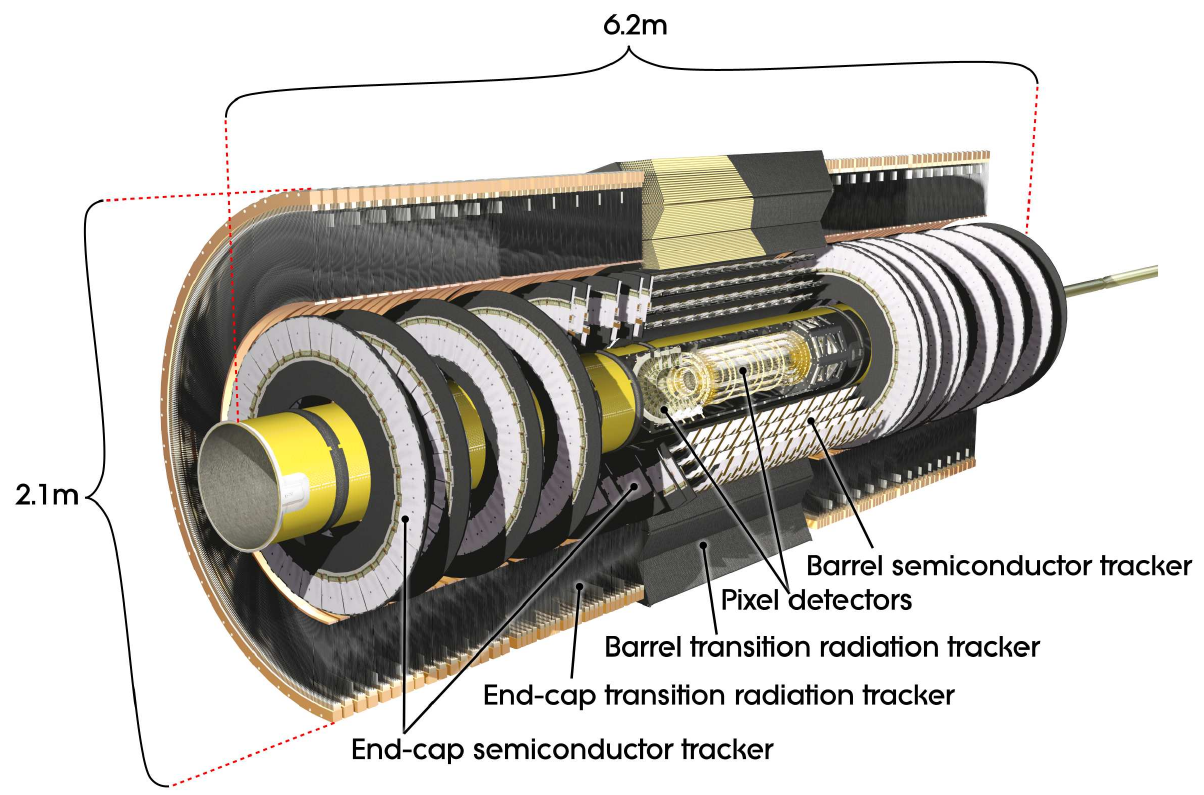
\includegraphics[width=\linewidth,height=\textheight,keepaspectratio]{atlas/inner_detector_xsec}
        \caption{Cutaway view of the Inner Detector sub-system \cite{atlas_tdr}}
        \label{fig:inner_detector_xsec}
    \end{figure}

    \begin{table} \centering
\caption{General specifications of Inner Detector modules \cite{atlas_tdr} \cite{insertable_Blayer}.}
\label{tab:ID_specs}
\begin{tabular}{ |l l|l|l| }
    \hline
    \textbf{Item}                   & &       \textbf{Radial extension (mm)} & \textbf{Length (mm)} \\
    \hline
    \textbf{Overall ID envelope}    & &         \textbf{0 < R < 1150}        &\textbf{0 < |z| < 3512} \\
    Beam-pipe                       & &            29 < R < 36    & \\
    \hline

    \textbf{IBL}          &  Overall envelope  &  31.0 < R < 40.0          &             \\    
                          &  Sensitive barrel  &  <R> = 25.7               &  |z| < 332 \\    
    &&&\\
    \textbf{Pixel}        &  Overall envelope  &  45.5 < R < 242           &  0 < |z| < 3092 \\
    3 cylindrical layers  &  Sensitive barrel  &  50.5 < R < 122.5         &  0 < |z| < 400.5 \\
    2 × 3 disks           &  Sensitive end-cap &  88.8 < R < 149.6         &  495 < |z| < 650 \\
    &&&\\
    \textbf{SCT}          &  Overall envelope  &  255 < R < 549 (barrel)   &  0 < |z| < 805 \\
                          &                    &  251 < R < 610 (end-cap)  &  810 < |z| < 2797 \\
    4 cylindrical layers  &  Sensitive barrel  &  299 < R < 514            &  0 < |z| < 749 \\
    2 × 9 disks           &  Sensitive end-cap &  275 < R < 560            &  839 < |z| < 2735 \\
    &&&\\
    \textbf{TRT}          &  Overall envelope  &  554 < R < 1082 (barrel)  &  0 < |z| < 780 \\
                          &                    &  617 < R < 1106 (end-cap) &  827 < |z| < 2744 \\
    73 straw planes       &  Sensitive barrel  &  563 < R < 1066           &  0 < |z| < 712 \\
    160 straw planes      &  Sensitive end-cap &  644 < R < 1004           &  848 < |z| < 2710 \\
    \hline
\end{tabular} \end{table}



    \subsection{Pixel Detector and Semiconductor Tracker}
        % purpose
        As the very first detector elements that any particles leaving the interaction region will encounter, the Pixel Detector and SCT face a precarious dilema.
        On the one hand, they must be able to accurately track the path of all ionizing particles emerging from the IR at high resolution (see table \ref{tab:ID_resolution}).
        On the other hand, any disturbance they introduce to particle trajectories will distort the measurment from every other detector in ATLAS.
        Add to this that these detectors face the highest radiation flux of any system simply by their proximity to the IR, forcing usage of very radiation-hard material design.
        For these reasons, the Pixel Detector and SCT use top-of-the-line silicon semiconductor diode technology, which can be made both extremely thin and sensitive. 
        This means that particles only deposit a small fraction of their energy into the detector material, and yet that small deposition is enough to accurately record their passage.
        With three layers of the Pixel Detector and four of the SCT, any particle leaving the IR crosses at least seven detector layers, yet continues on with a mostly unchanged trajectory.

        \begin{table}[] \centering \footnotesize
\caption{Resolution of the various Inner Detector Modules \cite{id_tdr}\cite{insertable_Blayer}.}
\label{tab:ID_resolution}
\begin{tabular}{|l|l|l|l|l|l|}
\hline
\textbf{System} & \textbf{Position} & \textbf{ Area }                 & \textbf{ Resolution }   & \textbf{ Channels } & \textbf{$\eta$} \\
\textbf{}       & \textbf{        } & \textbf{(m\textsuperscript{2})} & \textbf{\sigma($\mu$m)} & \textbf{ ($10^6$) } & \textbf{Coverage} \\
\hline
Pixels         & 1 insertable barrel layer & 0.38      & $R\phi$ = 50, z = 250    & 13.2           & $\pm 3  $       \\
               & 1 removable barrel layer  & 0.2       & $R\phi$ = 12, z = 66     & 16             & $\pm 2.5$       \\
               & 2 barrel layers           & 1.4       & $R\phi$ = 12, z = 66     & 81             & $\pm 1.7$       \\
               & 4 end-cap disks           & 0.7       & $R\phi$ = 12, R = 77     & 43             & 1.7-2.5         \\
               & on each side              &           &                          &                &                 \\
Silicon strips & 4 barrel layers           & 34.4      & $R\phi$ = 16, z = 580    & 3.2            & $\pm 1.4$       \\
               & 9 end-cap wheels          & 26.7      & $R\phi$ = 16, R = 580    & 3.0            & 1.4–2.5         \\
               & on each side              &           &                          &                &                 \\
TRT            & Axial barrel straws       &           & 170 (per straw)          & 0.1            & $\pm 0.7$       \\
               & Radial end-cap straws     &           & 170 (per straw)          & 0.32           & 0.7–2.5         \\
               & 36 straws per track       &           &                          &                &                 \\
\hline
\end{tabular} \end{table}


        Semiconductor diode detectors function by exploiting the properties of semiconductor p-n junctions.
        These particular detectors are made using silicon.
        Silicon has four valence electrons, so a pure silicon crystal lattice will have its valence band perfectly filled, leading to a very stable structure.
        A pure semiconductor crystal lattice (in this case, silicon) can have impurities intentionally introduced to it through the process of doping.
        Doping the lattice with an element possesing only three valence electrons (e.g. Boron) will result in a number of gaps in the valence band (called "holes").
        In such a situation, known as p-type doping, the lattice will accept additional electrons to fill these holes, which will lead to an excess of negatively charged ions.
        Conversly, an element with five valence electrons can be introduced for doping, leading to an excess of electrons in the valence band.
        Known as n-type doping, such an excess results in a lattice with a propensity for shedding these excess valence electrons, which in turn leads to an excess of positive ions.
        A p-n junction can be produced by taking a single silicon wafer and n-type doping one half, while p-type doping the other.
        The junction where the two dopings meet will then see a transfer of excess valence electrons moving from the n-type side to fill the holes of the p-type side, as illustrated in figure \ref{fig:pn_junction}

        \begin{figure}
            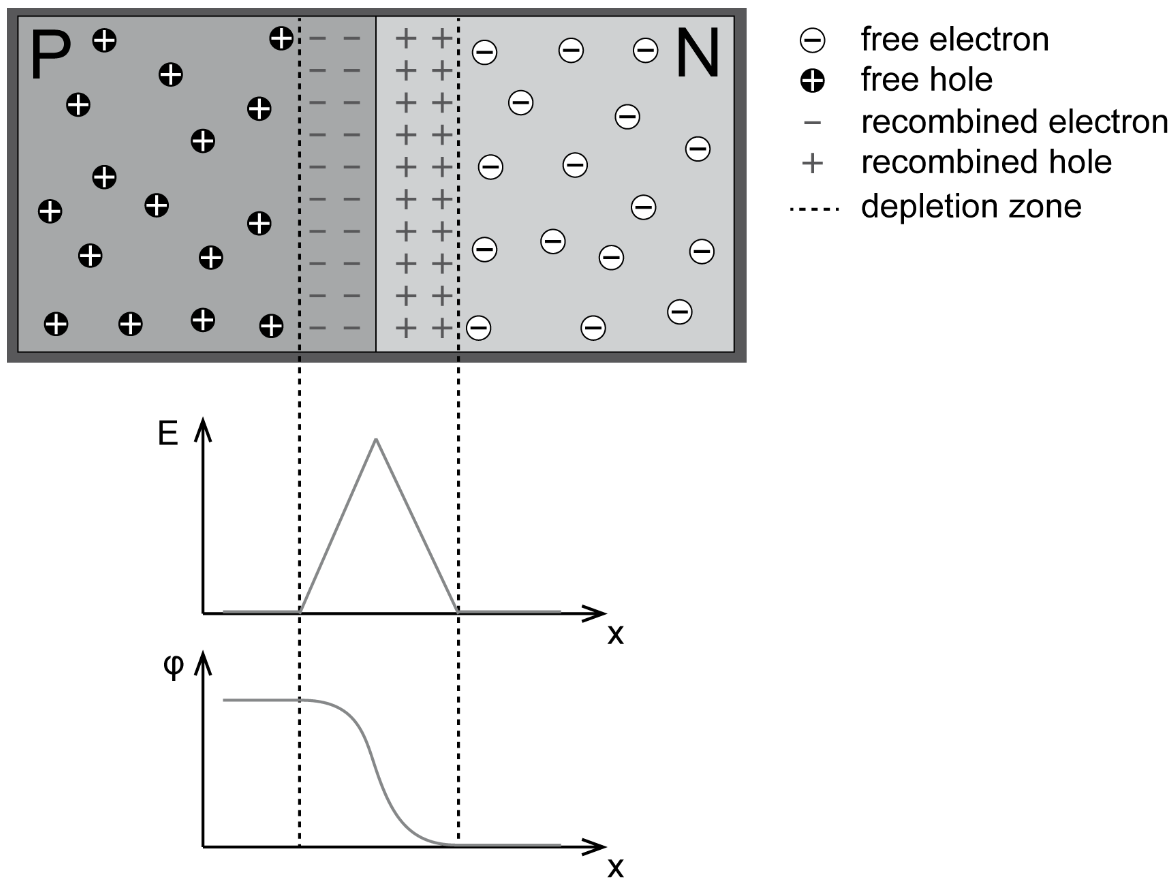
\includegraphics[width=\linewidth,height=\textheight,keepaspectratio]{atlas/pn_junction}
            \caption{Representation of a p-n junction, its depletion region, and the electric field and potential across its surface \cite{Havránek:2317324}}
            \label{fig:pn_junction}
        \end{figure}

        As the excess "donor" electrons migrate to fill the "acceptor" holes, the area around the junction has its valence band filled, creating an area called the "depletion zone".
        Though the depletion zone has a filled valence band, it has done so at the cost of ionization; an excess of electrons now populates the p-type side, with an equal number of positive ions remaining on the n-type side.
        The depletion zone grows larger until the migration of holes and electrons is balanced by the electric potential created through this ionization.
        When equilibrium is achieved, the lattice is left with an electric potential which monotonically decreases from the n-type to the p-type side, and which spans the full width of the depletion zone (refer again to figure \ref{fig:pn_junction}).
        If a voltage is applide across the semiconductor, the width and potential difference of the depletion region can be altered.
        If the voltage is applied with the positive end of the difference at the p-type side, then the semiconductor is said to be "forward biased", and the depletion region will become smaller (and with a high enough voltage can be eliminated entirely).
        If the positive end of the voltage difference is applied to the n-type side though, the semiconductor becomes "reverse biased", and the depletion region and potential difference across the junction will grow larger \cite{wiley_radiation_detection}.
        In this reverse-biased state, the electric potential of the p-n junction becomes very effective at rapidly sweeping excess ions from the depletion region off to the edges of the semiconductor wafer, and it is this mechanism which the ATLAS semiconductor detectors exploit in order to detect particles.

        Ionizing radiation is any particle that interacts electromagnetically, which means either photons or any particle with electric charge.
        When ionizing radiation passes through an element of the Pixel Detector or SCT, it will momentarily separate electrons from their nuclei in the silicon lattice.
        Normally, such separated ions would just recombine in a matter of moments.
        Because of the electric potential in the depletion region though, these ions are further seperated, and swiftly arrive at opposite ends of the semiconductor wafer.
        The very leads responsible for biasing the semiconductor are then responsible for collecting these seperated ions, which will cause a sudden jump in the circuit's current.
        The electric current through these semiconductor detectors is closely monitored, and these spikes are used to identify the passage of a particle through the semiconductors.

    \subsection{Transition Radiation Tracker (TRT)}
            Where the Pixel Detector and SCT focus on quality over quantity in their tracking, the TRT serves to take the opposite approach.
            The TRT has a resolution much lower than that of either the Pixel or SCT.
            But where the Pixel and SCT combined only manage about seven recorded hits per particle, the TRT achieves around 36.
            High statistics then are able to offset the TRT's lower resolution per hit, overall achieving a similar uncertainty on its track measurments.
            Such measurement needs to be accomplished under the same restrictions faced by the earlier trackers though.
            Namely, that it must obtain these measurements while causing minimal deviation in particle trajectory and also tolerating heavy radiation exposure over time.
            These challenges and goals are addressed in the TRT's composition, using a detector technology known as ``proportional drift tubes".

            The TRT consists of a large number of proportional drift tubes, often referred to as ``straws".
            Proportional drift tubes function in a similar way to semiconductor diode detectors, but using a gas instead of a doped semiconductor.
            The primary component of a drift tube is a cylinder filled with a gas mixture.
            In the TRT, these cylinders are 4 mm in diameter, filled with a mixture of 70\% Xenon, 27\%CO\textsuperscript{2}, and 3\% O\textsuperscript{2}.
            Ions are produced in this mixture when ionizing radiation passes through it.
            As in the semiconductor diode detectors, these ions are collected by applying an electric field through the ionization medium in order to sweep ions away into external circutry for readout.
            In a drift tube this is accomplished by maintaining an electric potential between the tube wall and a conductive wire running through the cylinder axis \cite{drift_chambers}.
            %NOTE: do I need to mention avalanche multiplication?
            The wall of the tube acts as the positively charged anode to collect electrons produced by the ionization, while the axial wire is kept at high electrical potential to act as the cathode.
            In the TRT, the cathode wall is made of aluminium and the 30 $\mu$m diameter anode wire of gold-plated tungsten. \cite{trt_design}

            \begin{figure}
                \begin{subfigure}{.48\textwidth}
                    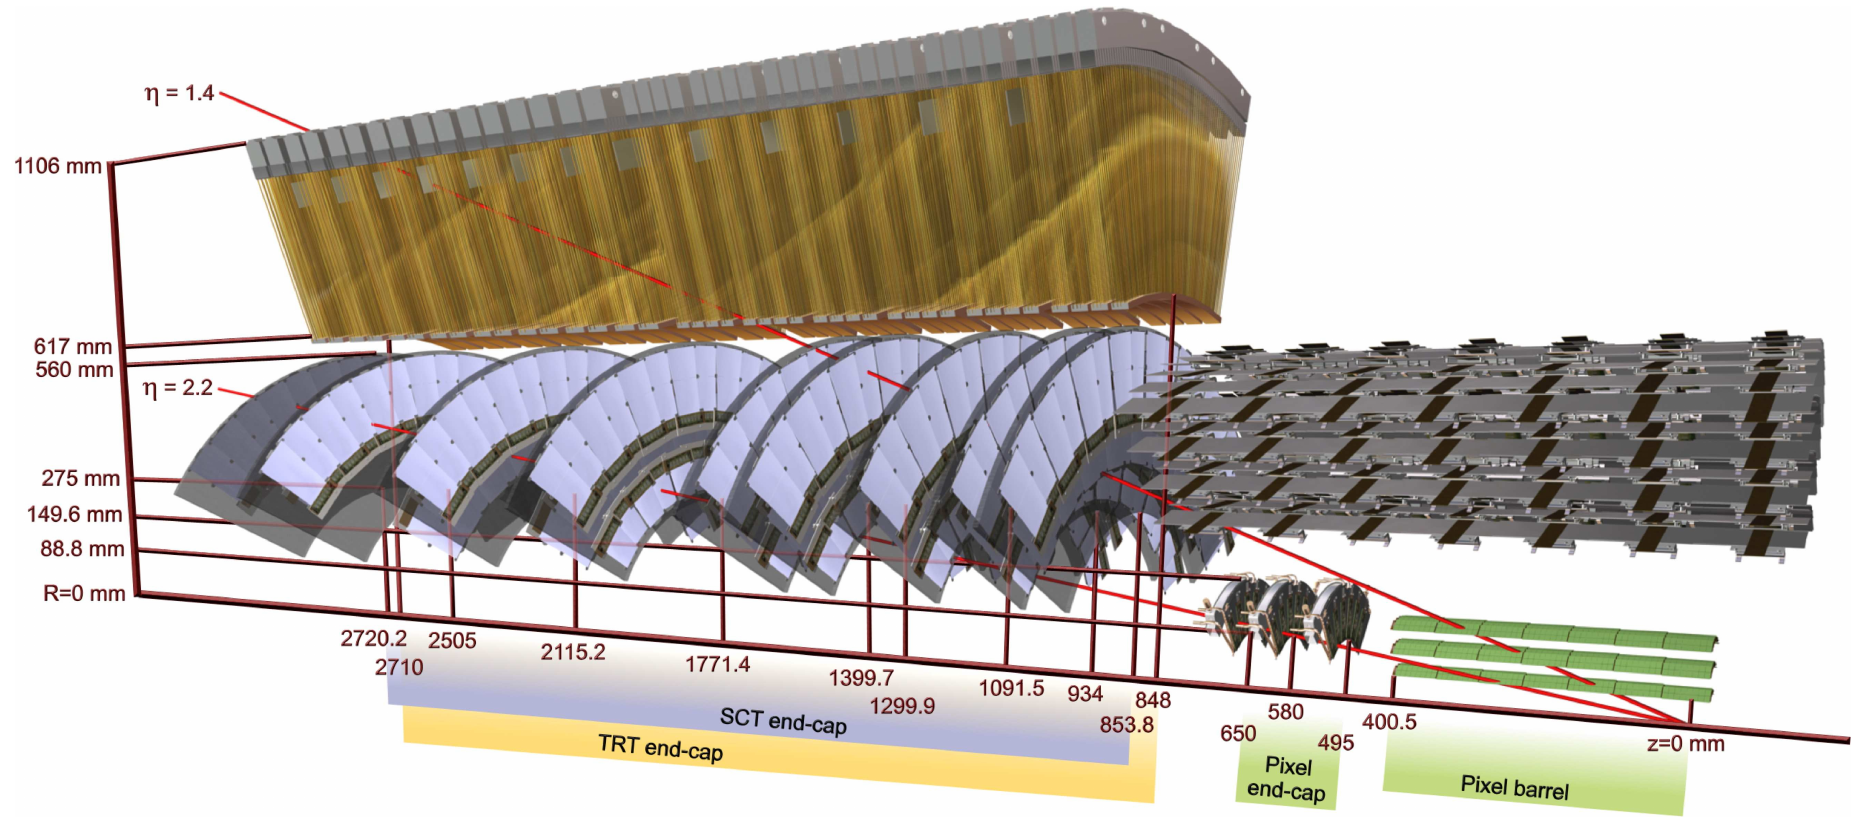
\includegraphics[width=\linewidth,height=\textheight,keepaspectratio]{atlas/inner_detector_endcap_measurements}
                    \caption{ID Endcap}
                    \label{fig:inner_detector_endcap_measurements}
                \end{subfigure}
                \begin{subfigure}{.48\textwidth}
                    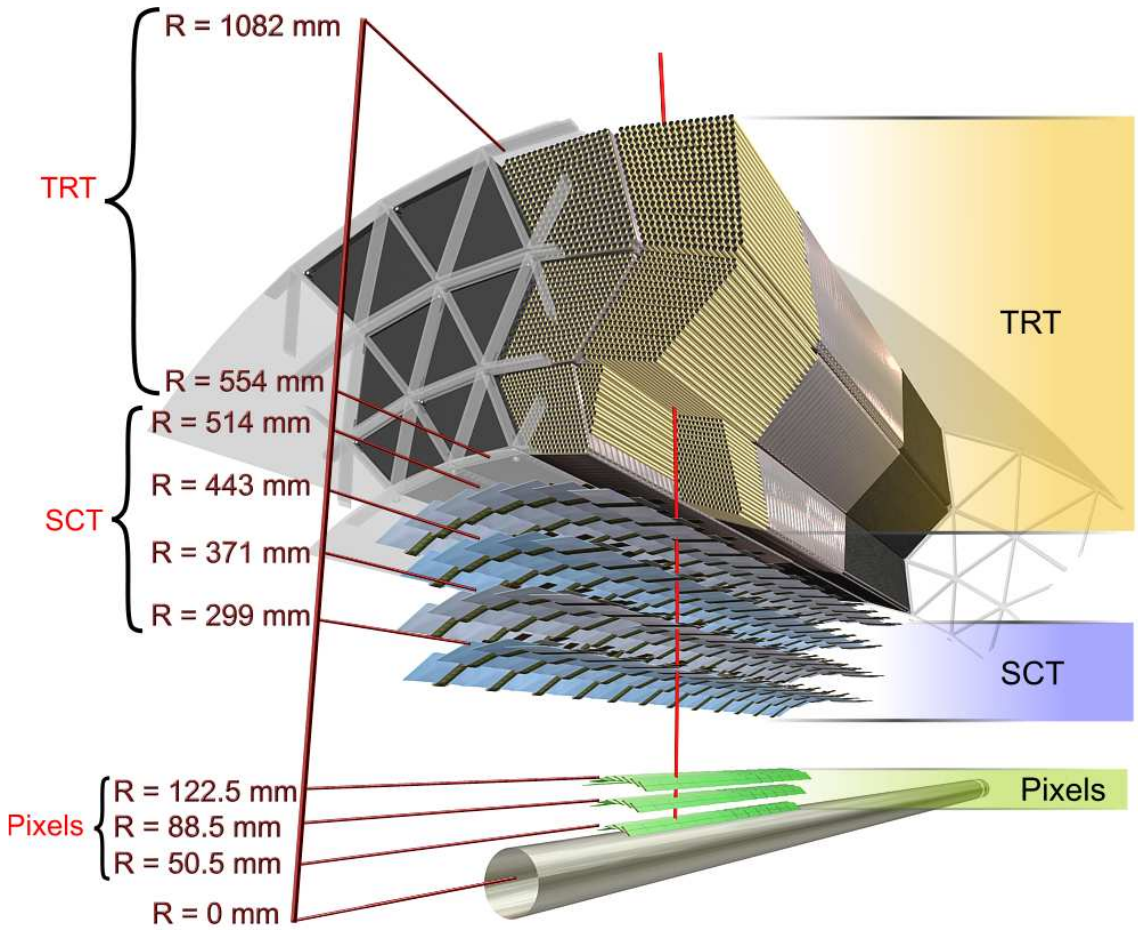
\includegraphics[width=\linewidth,height=\textheight,keepaspectratio]{atlas/inner_detector_barrel_measurements}
                    \caption{ID Barrel}
                    \label{fig:inner_detector_barrel_measurements}
                \end{subfigure}
                \caption{Visualization of the Inner Detector modules with corresponding measurments \cite{atlas_tdr}}
                \label{fig:inner_detector_measurements}
            \end{figure}

            For the TRT barrel, there are 52,544 straws 144 cm in length, while the endcaps each contain 122,880 straws 37 cm in length.
            These straws are arranged parallel to the beampipe in the barrel, and orthogonal to the beampipe in the endcap (see figure \ref{fig:inner_detector_measurements}).
            This arrangment is to maximize the number of straws traversed by an outgoing particle, typically 35-40 straws for $0 < |\eta| < 2$.
            Though each individual hit has a relatively low spatial resolution compared to the semiconductor detectors, the large number of hits compensates for this with a reduced statistical uncertainty.

            In addition to providing additional tracking information, the TRT provides a secondary purpose of aiding in the identification of electrons by means of detecting transition radiation. 
            Transition radiation is a phenomenon in which radiation is emitted when a charged particle crosses a boundary between two materials \cite{transition_radiation}.
            The TRT uses polypropylene as its transition radiation material, which is interleaved between the layers of straws.
            In the barrel, there are 73 layers of straws interwoven with polypropylene fibres, and in the endcaps there are 160 layers of straws with polypropylene foil between them.
            The large number of layers provide ample and repeated oppurtunity for charged particles crossing the TRT to encounter transition layers and emit identifying radiation, which is later used to distinguish electrons from other ionizing radiation.


\section{Calorimetry} \label{sec:calorimeter}
    The ATLAS Calorimeter system is designed to measure the energy of particles emerging from the Interaction Region.
    The entire collection of sub-detectors extends from the immediate outer edge of the Inner Detector region, out to a radius of 4.25 m, and longitudinally out to 6.12 m.
    Together the various systems achieve complete measurment coverage out to $|\eta| < 4.9$.

    There are a number of different ways to measure the energy of a particle, but in ATLAS this is done exclusively using the class of calorimeters known as \textit{sampling} calorimeters.
    Fundamentally, particle calorimeters work by impeding the path of a particle with some material, such that the particle is forced to interact with that material and deposit energy into it.
    This interaction must be such that it produces a measurable response, proportional to the deposited energy.
    A sampling calorimeter functions by measuring only a fraction of the deposited energy, spread out across the detector medium; i.e. by taking a sample of the energy.
    To do this, two different materials are used in the detector's construction, reffered to as the active and inactive materials.
    The active material is the material which actually measures the energy of particles, using the same or similar techniques as the tracking systems discussed earlier.
    The inactive material in turn has no detection capababilities, but is instead meant purely for the purpose of the aforementioned impedence of particle trajectories.
    Typically, inactive calorimeter material is a very dense and heavy high $Z$ medium, in order to maximize the number of particle interactions per unit distance.
    The active and inactive materials are arranged in alternating layers, so that the active material gets a snapshot of the way the particle is depositing energy across the entire length of the detector.\cite{energy_measurement}

    \begin{figure}
        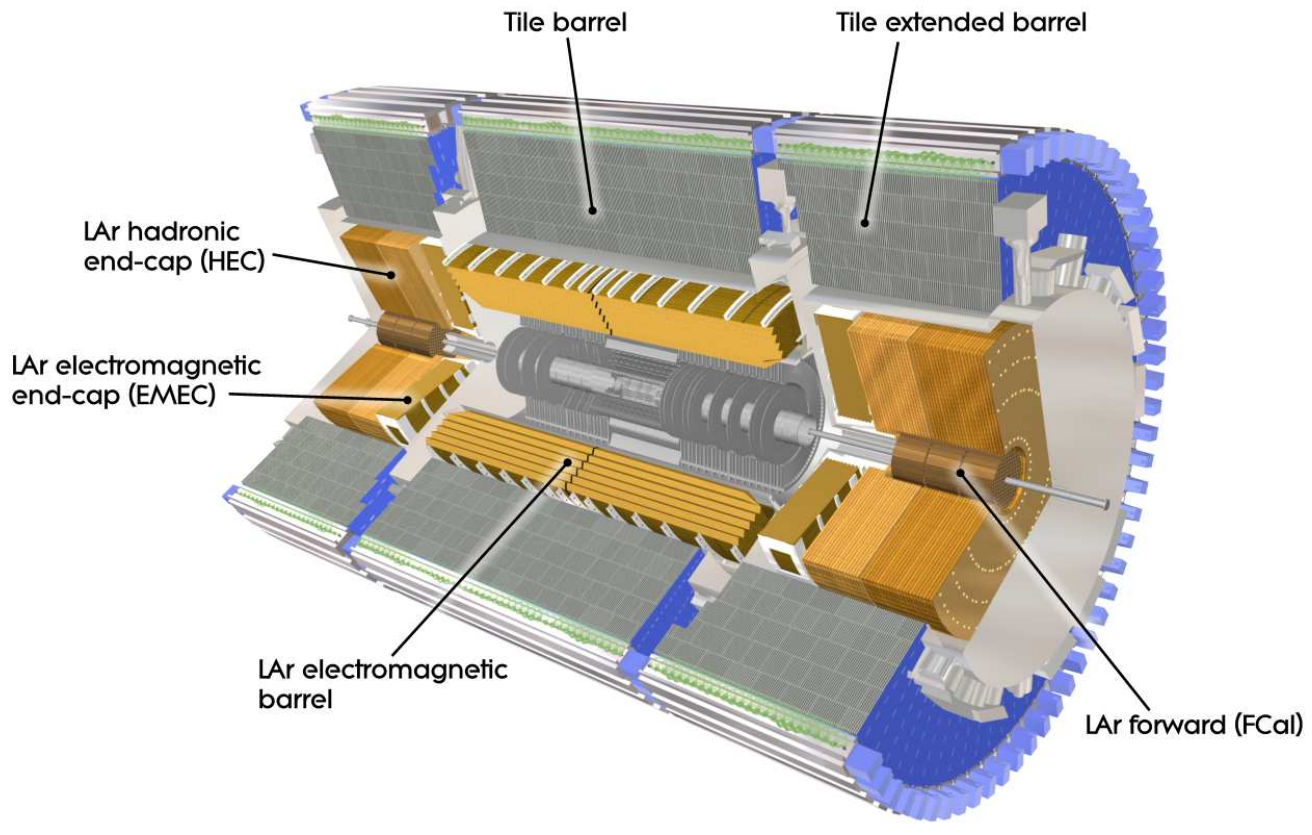
\includegraphics[width=\linewidth,height=\textheight,keepaspectratio]{atlas/cal_xsec}
        \caption{Cutaway view of the Calorimetry sub-system \cite{atlas_tdr}}
        \label{fig:cal_xsec}
    \end{figure}

    The Calorimetry system is split among three different subsystems, designed to measure two distinct kinds of particles.
    The innermost of these subsystems is the Electromagnetic Calorimeter (ECal), designed primarily to measure (anti) electrons and photons \cite{calorimetry_lecture}.
    These particles readily interact electromagnetically in the calorimeter material, rapidly losing energy and permitting the ECal to be more compact.
    Surrounding the ECal are the Hadronic Calorimeter (HCal) systems.
    These detectors, as their name suggests, detect hadrons, such as neutrons or pions.
    Not only are these particles heavier, but many of them are electrically neutral and can therefore only be stopped through repeated nuclear interactions \cite{energy_measurement}.
    Consequently, the HCal systems are significantly thicker and use more dense inactive materials that that of the ECal (see figure \ref{fig:cal_rad_length}).
    \begin{figure}
        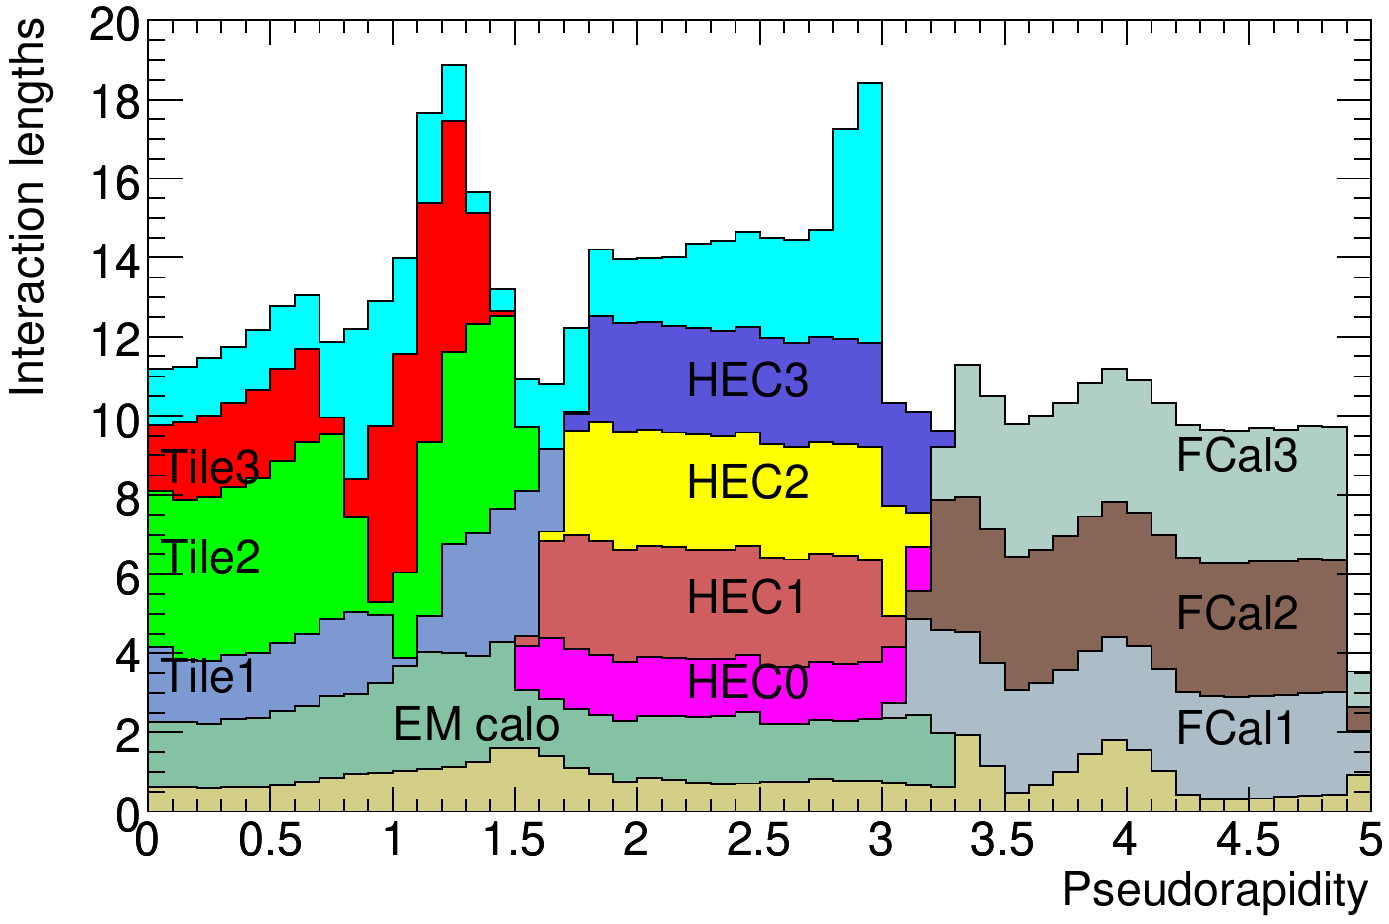
\includegraphics[width=\linewidth,height=\textheight,keepaspectratio]{atlas/cal_rad_length}
        \caption{Histogram of interaction lengths $X_0$ as a function of $\eta$ for the different sub-detectors \cite{atlas_tdr}}
        \label{fig:cal_rad_length}
    \end{figure}
    Additionally, they serve the crucial role of preventing hadrons from escaping into the Muon Spectrometer.
    The final subsystem of the Calorimetry system is the Forward Calorimeter (FCal).
    The FCal records, across different sections, the energy of electromagnetic and hadronic particles.
    It is constructed very close to the beampipe, and serves to extend the calorimetric measurement coverage out to an $|\eta|$ of 4.9.

    \subsection{Electromagnetic Calorimeters}
        Purpose is to detect electrons and photons at high resolution.
        Both barrel and encaps use lead as their inactive material, and Liquid Argon as the active material.
        The liquid argon calorimeters, used in the ECal and elsewhere, detects ionization from incident particles via capacitive coupling to electrodes placed outside the active medium.
        Liquid argon as the active medium in particular is used because of its intrinsic radiation hardness and linear ionization response to radiation \cite{Lar_cal_tdr}.
        Uses a unique "accordian" design in the layout of the material layers, in order to provide complete coverage in $\phi$.
        Also uses a "Presampler", due to an excess of material in front of the ecal.
        Presampler needed to account for energy lost in this material


    \subsection{Hadronic Calorimeter}
        Serves to detect hadrons, and to prevent "punch-through" into the Muon System.
        The Hadronic Endcap Calorimeter (HEC) uses Liquid Argon for the active material, like the ECals, but uses copper plates for the inactive material.
        The HCal Barrel, referred to as the Tile Calorimeter, uses steel plates as the inactive material, and scintillating tiles as the active material.
        The scintillating tiles used here operate on different electrical principles than the LAr detectors used across the other calorimeters.
        The key to scintillating materials is that they respond to ionizaing radiation by fluorescing.
        That is, when ionizing radiation crosses through the scintillation material, the material momentarily enters an excited state.
        The excited material promptly returns to its base energy state, and releases the excess energy in the form of photons, called "scintillation light".
        Ideally, this flourescent response is related to the energy of the incident radiation through as linear a response as possible \cite{wiley_radiation_detection}.
        In the Tile Calorimeter, the scintillating material used is polystyrene, and the energy itself is measured by transferring the light to optical fibres located at the edge of the tile modules.
        These optical fibres direct the light to photomultiplier tubes (PMTs), which in turn convert the light to electrical signals to be read out \cite{tcal_tdr}.


    \subsection{Forward Calorimeter}
        Purpose is to extend calorimetry coverage as far as $|\eta| < 4.9$.
        Divided into three parts: 1 ECal, and 2 HCals
        All parts use LAr for active medium, but ECal uses copper while Hcals use Tungsten for inactive medium
        Exposed to extremely high radiation flux, necessitating materials that are both very dense and very radiation-resistant \cite{Lar_cal_tdr}.

    \begin{table}[] \tiny \centering
\caption{General specifications of calorimeter systems \cite{atlas_tdr}.}
\label{tab:cal_specs}
\begin{tabular}{|l|lc|lc|}
\hline 
                                               &                  \multicolumn{2}{c|}{\textbf{Barrel}}            &           \multicolumn{2}{c|}{\textbf{End-cap}}                                 \\
\hline 
                                               \multicolumn{5}{|c|}{\textbf{EM Calorimeter}} \\
\hline 
                                               \multicolumn{5}{|c|}{Number of layers and $|\eta|$ coverage} \\
\hline 
Presampler                                     & 1                 & $|\eta|$ < 1.52                 & 1                               & 1.5 < $|\eta|$ < 1.8     \\
Calorimeter                                    & 3                 & $|\eta|$ < 1.35                 & 2                               & 1.375 < $|\eta|$ < 1.5   \\
                                               & 2                 & 1.35 < $|\eta|$ < 1.475 & 3                                       & 1.5 < $|\eta|$ < 2.5     \\
                                               &                   &                                 & 2                            & 2.5 < $|\eta|$ < 3.2     \\
\hline 
                                               \multicolumn{5}{|c|}{Granularity $\Delta \eta \times \Delta \phi$ versus $|\eta|$} \\
\hline 
Presampler                                     & 0.025 × 0.1       & $|\eta|$ < 1.52                 & 0.025 × 0.1                     & 1.5 < $|\eta|$ < 1.8     \\
Calorimeter 1st layer                          & 0.025/8 × 0.1     & $|\eta|$ < 1.40                 & 0.050 × 0.1                     & 1.375 < $|\eta|$ < 1.425 \\
                                               & 0.025 × 0.025     & 1.40 < $|\eta|$ < 1.475 & 0.025 × 0.1                             & 1.425 < $|\eta|$ < 1.5   \\
                                               &                   &                                    & 0.025/8 × 0.1                   & 1.5 < $|\eta|$ < 1.8     \\
                                               &                   &                                    & 0.025/6 × 0.1                   & 1.8 < $|\eta|$ < 2.0     \\
                                               &                   &                                    & 0.025/4 × 0.1                   & 2.0 < $|\eta|$ < 2.4     \\
                                               &                   &                                    & 0.025 × 0.1                     & 2.4 < $|\eta|$ < 2.5     \\
                                               &                   &                                    & 0.1 × 0.1                       & 2.5 < $|\eta|$ < 3.2     \\
\hline 
Calorimeter 2nd layer                          & 0.025 × 0.025     & $|\eta|$ < 1.40                    & 0.050 × 0.025                   & 1.375 < $|\eta|$ < 1.425 \\
                                               & 0.075 × 0.025     & 1.40 < $|\eta|$ < 1.475 & 0.025 × 0.025                              & 1.425 < $|\eta|$ < 2.5   \\
                                               &                   &                                    & 0.1 × 0.1                       & 2.5 < $|\eta|$ < 3.2     \\
\hline 
Calorimeter 3rd layer                          & 0.050 × 0.025     & $|\eta|$ < 1.35                 & 0.050 × 0.025                   & 1.5 < $|\eta|$ < 2.5     \\
\hline 
                                               \multicolumn{5}{|c|}{Number of readout channels} \\
\hline 
Presampler                                     & 7808              &                                    & 1536 (both sides)               &                                     \\
Calorimeter                                    & 101760            &                                    & 62208 (both sides)              &                                     \\
\hline 
                                               \multicolumn{5}{|c|}{\textbf{LAr Hadronic End-cap}} \\
\hline 
$|\eta|$ coverage                              &                   &                                    & 1.5 < $|\eta|$ < 3.2 &                                     \\
Number of layers                               &                   &                                    & 4                               &                                     \\
\hline 
Granularity $\Delta \eta \times \Delta \phi$   &                   &                                    & 0.1 × 0.1                       & 1.5 < $|\eta|$ < 2.5     \\
                                               &                   &                                    & 0.2 × 0.2                       & 2.5 < $|\eta|$ < 3.2     \\
\hline 
Readout channels                               &                   &                                    & 5632 (both sides)               &                                     \\
\hline 
                                                       \multicolumn{5}{|c|}{\textbf{LAr Forward Calorimeter}} \\
\hline 
$|\eta|$ coverage                              &                   &                                    & 3.1 < $|\eta|$ < 4.9 &                                     \\
Number of layers                               &                   &                                    & 3                               &                                     \\
\hline 
Granularity $\Delta x \times \Delta y$ (cm)    &                   &                                    & FCal1: 3.0 × 2.6                & 3.15 < $|\eta|$ < 4.30   \\
                                               &                   &                                    & FCal1: \~ four times finer       & 3.10 < $|\eta|$ < 3.15,  \\
                                               &                   &                                    &                                 & 4.30 < $|\eta|$ < 4.83   \\
                                               &                   &                                    & FCal2: 3.3 × 4.2                & 3.24 < $|\eta|$ < 4.50   \\
                                               &                   &                                    & FCal2: \~ four times finer       & 3.20 < $|\eta|$ < 3.24,  \\
                                               &                   &                                    &                                 & 4.50 < $|\eta|$ < 4.81   \\
                                               &                   &                                    & FCal3: 5.4 × 4.7                & 3.32 < $|\eta|$ < 4.60   \\
                                               &                   &                                    & FCal3: \~ four times finer       & 3.29 < $|\eta|$ < 3.32,  \\
                                               &                   &                                    &                                 & 4.60 < $|\eta|$ < 4.75   \\
\hline 
Readout channels                               &                   &                                    & 3524 (both sides)               &                                     \\
\hline 
                                               \multicolumn{5}{|c|}{\textbf{Scintillator Tile Calorimeter}} \\
\hline 
                                               & Barrel            &                                    & Extended barrel                 &                                     \\
\hline 
$|\eta|$ coverage                              &    $|\eta|$ < 1.0 &                                    & 0.8 < $|\eta|$ < 1.7 &                                     \\
Number of layers                               & 3                 &                                    & 3                               &                                     \\
\hline 
Granularity $\Delta \eta \times \Delta \phi$   & 0.1 × 0.1         &                                    & 0.1 × 0.1                       &                                     \\
Last layer                                     & 0.2 × 0.1         &                                    & 0.2 × 0.1                       &                                     \\
\hline 
Readout channels                               & 5760              &                                    & 4092 (both sides)               &                                    \\
\hline 
\end{tabular} \end{table}




\section{Muon Spectrometer} \label{sec:muon}
    The Muon Spectrometer has the purpose of providing track position and momentum measurements for muons exiting the ATLAS detector.
    The Muon barrels start at a radii of 5 m from the beam axis, extending out to 10 m.
    The endcaps start at a $|z|$ of roughly 7.4 m, and proceed to an extent of 21.5 m.
    The immense size of the muon system poses a challenge, as it must provide tracking across its entire volume.
    %Its distance from the interaction point ameliorates this issue though, as it permits the Muon detectors to operate at much lower spatial resultions than the inner detectors, while still retaining similar anngular resolution.

    \begin{figure}
        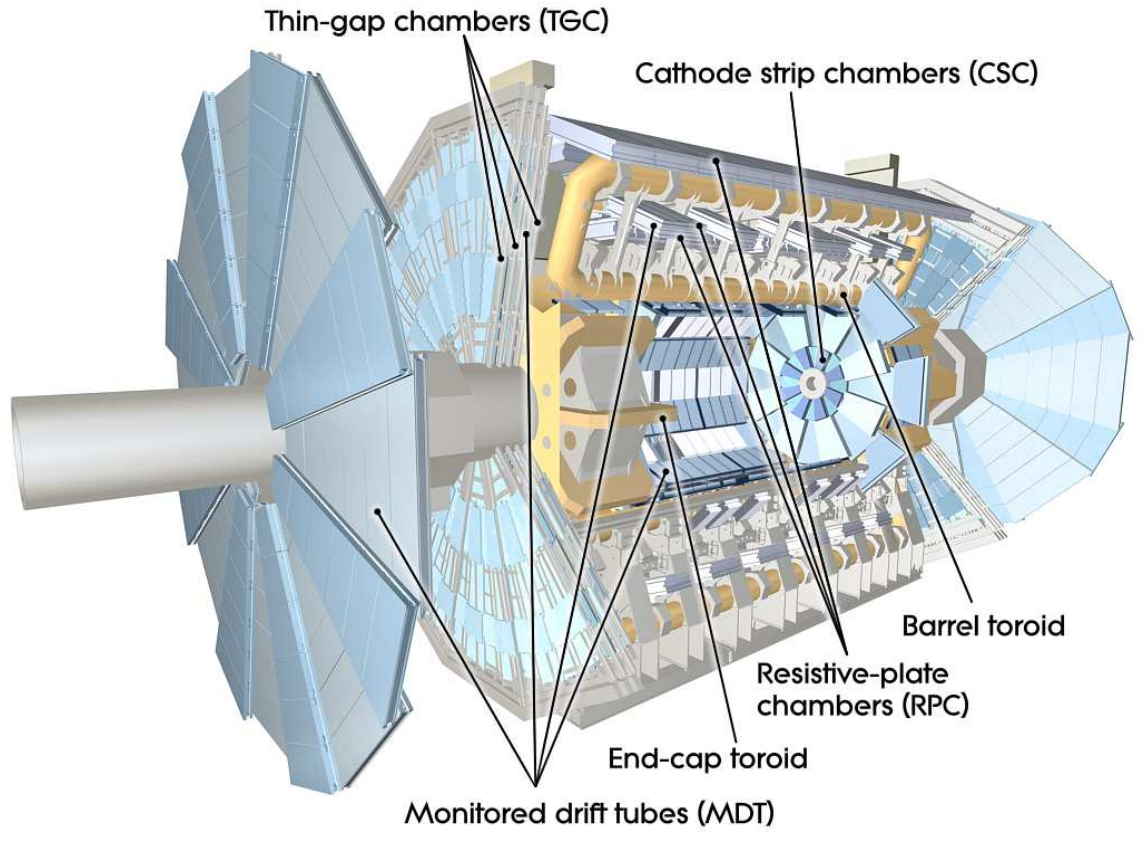
\includegraphics[width=\linewidth,height=\textheight,keepaspectratio]{atlas/muon_xsec}
        \caption{Cutaway view of the Muon Spectrometer \cite{atlas_tdr}}
        \label{fig:muon_xsec}
    \end{figure}

    \subsection{Toroid magnets}
        Three large air-core toroids meant to deflect muons.
        Barrel provides 1.5-5.5 Tm (Tesla-meters???) of bending power in $0<|\eta|<1.4$,
        and endcaps provide 1-7.5 Tm in $1.6<|\eta|<2.7$.
        The power is lower in the region where the fields overlap ($1.4<|\eta|<1.6$)

    \subsection{Precision Track Chambers}
        The Precision Track Chambers are designed to provide high resolution measurements of track position and momentum for particles escaping the ATLAS detector. Split across two technologies, the Monitored Drift Tube Chambers (MDT's) and Cathode-Strip Chambers (CSC's).
        The MDT's are drift tube chambers (like the earlier TRT, but larger) filled with Ar/CO2 gas using a tungsten-rhenium wire for charge collection. These are used in both the barrel and endcap regions, covering the range $|\eta| < 2.7$.
        The MDT consists of three endcap and three barrel layers, with a notable exception in the endcap region $2 < |\eta| < 2.7$.
        Within this $\eta$ range, for the first layer, the muon track density exceeds the resolution capabilities of the MDT's.
        As such, the first layer of the endcap in this range is replaced with CSC's.
        The CSC's are multiwire drift chambers, meaning that the (gold-plated tungsten) anode wires do not each have their own individual drift tube.
        Instead, each of the many drift chambers containes many anodes and many cathode strips, made of copper.
        These chambers can read both coordinates of a track simultaneosly, preventing the ambiguities that can occur if more than one track is present in the same chamber \cite{atlas_tdr}.

    \subsection{Trigger Chambers}
        Meant to provide rapid information on muon track multiplicity and energy range.
        Also provides additional track information for higher level triggers.
        Provides acceptance in range $|\eta| < 2.4$.
        The barrel and end-cap use two different technologies in order to address the different issues present in their respective regions.
        The barrel uses Resistive Plate Chambers (RPC's), which have higher temporal resolution.
        RPC's follow the same principle of operation as drift tube chambers, but the anode and cathodes are both conductive plates that maintain an electric potential in the gaseous mixture between them.
        The endcap consists of Thin Gap Chambers (TGC's), which are multi-wire drift tube chambers with very small gaps between the anode wires and the cathode strips; indeed, the anode-cathode gaps are 1.4 mm are smaller than the anode-anode gaps of 1.8 mm.
        The TGC serves to both tag beam-crossings and also deliver additional information on traversing particles' azimuthal coordinate, to complement the measurments of the MDT.

    \begin{table}[hb] \centering \scriptsize
\caption{General specifications of the Muon Spectrometer \cite{atlas_tdr}.}
\label{tab:muon_specs}
\begin{tabular}{|l|l|}
\hline
\textbf{Monitored Drift Tubes}    & \textbf{MDT}                                                      \\
- Coverage               & $|\eta|$ < 2.7 (innermost layer: $|\eta|$ < 2.0)         \\
- Number of chambers     & 1088 (1150)                                              \\
- Number of channels     & 339 000 (354 000)                                        \\
- Function               & Precision tracking                                       \\
\hline
\textbf{Cathode Strip Chambers}   & \textbf{CSC}                                                      \\
- Coverage               & 2.0 < $|\eta|$ < 2.7                                     \\
- Number of chambers     & 32                                                       \\
- Number of channels     & 31 000                                                   \\
- Function               & Precision tracking                                       \\
\hline
\textbf{Resistive Plate Chambers} & \textbf{RPC}                                                      \\
- Coverage               & $|\eta|$ < 1.05                                          \\
- Number of chambers     & 544 (606)                                                \\
- Number of channels     & 359 000 (373 000)                                        \\
- Function               & Triggering, second coordinate                            \\
\hline
\textbf{Thin Gap Chambers}        & \textbf{TGC}                                                      \\
- Coverage               & 1.05 < $|\eta|$ < 2.7 (2.4 for triggering)               \\
- Number of chambers     & 3588                                                     \\
- Number of channels     & 318 000                                                  \\
- Function               & Triggering, second coordinate                            \\
\hline
\end{tabular} \end{table}



% Ch4.5: ATLAS Trigger System - DRAFT 0
\chapter{Trigger System}

\section{Introduction}
    The amount of data output by the ATLAS detector is immense and overwhelming.
    Processing every single bunch crossing would require completely unphysical bandwidth levels, and would take centuries to process.
    To counteract this overabundance of data, ATLAS relies on its triggering system to drastically reduce its throughput.
    Known simply as the ATLAS trigger system, this critical piece of infrastructure constitutes the last step of data taking, and the first step of physics analysis.

    The trigger system is a series of hardware and software level algorithms designed to quickly identify bunch crossing ``events" which may be interest to physics analysis, while discarding the rest.
    Refered to as ``online" analysis, these algorithms perform event selection ``live" in parallel to the machine running and taking data.
    The trigger system processes all ATLAS events immediately after readout, ultimately reducing the 40 MHz bunch crossing rate to a data output rate of 1 kHz.
    The data which survives this rapid selection is read out to disk and distributed to individual research teams for more sophisticated ``offline" analysis later.
    
    Triggering is achieved by running events through two sequential trigger systems.
    All events first go through the hardware-based Level 1 Trigger (L1) before being being run through the more sophisticated (but slower) software-based High Level Trigger (HLT).
    Both of these triggers involve a plethora of different measurements on various aspects of the events, such as total transverse energy, transverse momentum, jet multiplicity, and opening angles between jets.
    Moreover, there is more than one possible way that an event can pass the trigger process.
    Each of the various kinematic properties the triggers determine have multiple threshold values that can determine a ``pass" (e.g. a jet $p_T$ trigger can have thresholds at 30, 45, or 55 GeV, among others).
    A ``trigger chain" is a combination of several different such kinematic conditions, each with their own thresholds.
    An bunch crossing is ultimately accepted and read out to disk for further analysis offline if it is able to pass all the conditions of a trigger chain.
    As stated earlier, there are several ways an event can pass the triggers, in the sense that there are a huge number of different trigger chains, each permitting a different combinations of permissable kinematics.
    An event is read out if it passes any one of the trigger chains, and is labelled in data with all the trigger chains it passes.
    All of the running trigger chains comprise the ``trigger menu".
    The chains included in the trigger menu were decided upon before the beginning of the Run 2 data taking period, based on input from various analysis teams.


\section{Level 1 Trigger}
    One bunch-crossing every 25 ns is a blistering pace to operate at.
    The first layer of the trigger system, L1, thus runs entirely through hardware-level gate logic.
    The goal of this system is to reduce the event rate from the raw 40 MHz bunch-crossing rate, down to a more manaegable rate of 100 kHz \cite{trigger_run2}.
    To reduce latency as much as possible, all the electronics comprising L1 are located as close as possible to ATLAS itself, specifically in the USA15 underground chamber \cite{trigger_tdr}.
    As yet another consequence of the high frequency L1 must operate at, it exclusively uses information from the ATLAS calorimeters and Muon Trigger Chamber for its decisions.
    %(utilizes detector buffer memory to keep up).

    The Muon Trigger aspect of L1 is based entirely around the trigger-dedicated Muon Trigger Chamber, which described in section. %\ref{sec:muon-trigger_chamber} FIXME uncomment 
    Its purpose is to make trigger decisions primarily based on muon $p_T$ and track multiplicity in the Trigger Chamber  \cite{trigger_run1}.
    In the calorimeter-based trigger, the selection algorithm involves the construction of key trigger objects that are crucial to understanding the events used in ATLAS analysis.

    The full granularity of the ATLAS calorimeters is too complex to analyze in the \textasciitilde 25 ns L1 has to process each bunch-crossing.
    Instead, the various sensors of the calorimeters are clustered together into ``trigger towers", each with a resolution of 0.1x0.1 in $\Delta \eta x \Delta \phi$.
    A ``Region of Interest" (RoI) is created as a group of towers which collectively satisfy the condition of a specific type of trigger.
    The way RoIs are formed and used varies between the different L1 calorimeter trigger modules: the CPM, JEM, and CMX.

    The Cluster Processor Module (CPM) exclusively uses the Barrel Calorimeters to function, and is primarily meant for rapid identification of electrons/photons and taus/hadrons.
    In either situation, the CPM's first step is to check all possible 4x4 ``windows" of trigger towers, identifying windows containing an isolated ``Region of Interest" (RoI).
    Here, an RoI is defined as a 2x2 cluster of towers with an $E_T$ sum that is a relative maximum compared to surrounding towers.
    This 2x2 RoI is the center of the 4x4 window (see figure [TODO INSERT FIGURE 13 OF L1_calo_run1]).
    Windows are considered as passing the CPM trigger if the RoI satisfies an isolation requirement, meaning that the 12 towers surrounding that core fall \textit{below} a predifined $E_T$ ``isolation threshold" value.
    Electrons and photons are then seperated from taus and hadrons by the fact that the latter group penetrates into the HCal barrel, while the former group stays highly contained to the ECal.

    Expanding out, the Jet/Energy Processing Module (JEM, or sometimes JEP) makes use of the calorimeter barrels and endcaps, as well as the FCAL, though it does not distinguish between the ECal and HCal.
    The JEM further reduces the granularity under consideration, with a basic unit of data collection being 2x2 collections of trigger towers called ``jet elements", resulting in minimum resolution of 0.2x0.2 in $\Delta \eta x \Delta \phi$.
    Like the CPM, the JEM runs its trigger conditions on windows of multiple jet elements that must be based around a 2x2 RoI core (which is a local $E_T$ maximum).
    Unlike the CPM, these windows can vary in size.
    Primarily, the JEM is intended to perform hit multiplicity counting as well as assist the Extended Cluster Merger Modules (CMX) in carrying out the final jet multiplicity and $E_T$ sums \cite{L1_calo_run1}\cite{trigger_run2}.


\section{High Level Trigger}
    After the L1 Trigger has reduced the event rate to 100 kHz, the software-based High Level Trigger (HLT) is used to further reduce the event rate to the final output of \textasciitilde 1 kHz.
    Located in the SCX1 building (TODO insert trigger_tdr figure 2) at the surface of P1 (again to minimize latency), the HLT uses data from all detector elements completely reconstruct the event as it occured in ATLAS, and performs its selections based on this reconstructed event.
    Different physics processes and particles, known as physics ``signatures", are reconstructed in different ways, and have different triggers based around them. 
    The main signatures used in ATLAS are: minimum bias signatures, electron/photons (Egamma), muons, jets, taus, missing transverse energy (MET), b-jets (as in jets from bottom quarks), and B-physics (as in B-hadrons).
    The process of reconstruction and the trigger algorithms applied to these reconstructed signatures are based on offline software algorithms.
    These offline algorithms are adjusted for use in the online environment, which is discussed further chapter [TODO].
    Once events have successfully passed both L1 and the HLT, they are finally distributed offsite for analysis by different physics groups.
    
    

% TODO: I think I'm going to move this into the "event reconstruction" chapter, since discussion of the retuning process is entirely based on discussion of the individual low-level and high-level algorithms used for the bjet trigger
%\section{HLT Retuning Framework}
%Finally something that I did!
%Except it didn't end up mattering...
%Do I need to mention specifically my work on the FTK? NOPE. Just talk about the retuning at a more general level.

  
% Ch5: How simulation and monte-carlo works (maybe a discussion of ATLAS software (Athena, ROOT, etc) too)?
%\chapter{Signal and Background Modeling}


\section{I'll figure this out later I just wanna jot this down for myself first}
    Here's my more formal attempt at writing down what I do in the 2/3D interpolation

    Overall goal is to measure cross-section of an interaction: $\Xsec \matel$
 %TODO

% Ch6: Search (what am I looking for, how did I go about it, etc) %TODO

% Ch7: Results (findings, uncertainties, statistics...) %TODO

% Ch8: Conclusion and Future Studies %TODO
%       work on ALTIROC

% appendix? (Steve said that last committee was not fond of too much stuff in appendix, pushed to just incorporate most of it into main body. Expect to do the same)

%\chapter{Printer Calibration}\label{chapter:printer_calibration}

As you may know, printers do not print your PDF file exactly.
They will scale it to match their own preset configurations and potentially add padding spaces around the edges.
There is no way to control for this as every printer is unique and there are no base standards.
The only thing a user can do is have their generated PDF file have the correct distances and then ask that the person printing their document calibrate the printer accordingly.

\printercalibration{}

\vspace{2in}
This chapter will provide printer calibrations.
All the \textcolor{red}{red lines} drawn are $1$~inch in length.
All the \textcolor{blue}{blue lines} drawn are $2$~inches in length.
These are drawn from the edge of the document in TikZ, which has good distance metrics built into it, so these distances are accurate.
Print this page and measure the margins and the length of the arrows.
If your measurements do not match those printed \textbf{you need to calibrate your printer}.
It is probable that your printer has an option that is along the lines of ``actual size'', so that might be a good starting point.
It can also help to turn on \verb|\geometry{showframe=true}| in your preamble.
 TODO: you should remember to use this eventually (thanks Matthew!)

\StartAppendix
    \chapter{An Appendix}\label{appendix:ATLAS_detector}

Appendix text goes here.


% Glossary
% Check with specific department on the style to use
\clearpage
\singlespacing%
\setglossarystyle{list}
\printglossary[title=GLOSSARY,toctitle=GLOSSARY]
\doublespacing%

% Bibliography goes below
% Check with specific department on the appropriate
% bibliography style to use

%\nocite{*}
\bibliographystyle{bib/JHEP}
\raggedright
\bibliography{bib/theory,bib/lhc,bib/atlas,bib/trigger}

\end{thesis}
\end{document}
